\chapter{Results}\label{chapter:results}
In the research community simplified synthetically generated datasets are quiet common for investigating underlying mechanisms and the applicability of different approaches for a given task. Of course, for the sake of completeness it is also necessary to test these approaches on the real-world task. Just if that is done properly one can estimate the robustness and therefore the actual benefit of the approach for the real-world task. In the following the results from different experiments on the dummy and the real-world dataset are described.

\section{Dummy dataset}
Several experiments were performed on the dummy dataset to analyze the effects of the MMD loss in an easy and clear setting and to make first estimates about its applicability for PHM. The models used are the same as described in section \ref{sec:model}. The model in \ref{cnn_mmd_dummy} was optimized as explained in section \ref{sec:Proposed_training}. In the experiments of section \ref{sec:Balancing Cross-Entropy and MMD loss} and \ref{sec:Differences of labeled and unlabeled MMD loss} just one SGD optimizer with learning rate 0.01 in combination with a weighted average between the MMD and source cross-entropy loss was used.

\subsection{Sensitive balancing of Cross-Entropy and MMD loss} \label{sec:Balancing Cross-Entropy and MMD loss}

In the following section, the sensitivity of the weighting factor GAMMA on the training is evaluated. The latent feature representation in FC2 for source and target domain is visualized in fig. \ref{fig:point_cloud_mmd}. The development of the MMD and cross entropy loss throughout the training is shown in fig. \ref{fig:learning_curves_influence_mmd_feature_extractor}.
\begin{itemize}
    \item \textbf{Small GAMMA}:
    When picking a very small GAMMA, the model is not able to generate a latent feature representation with a high compactness and separability between classes. Besides that, the class representations do not overlap well for the two domains. The domain discrepancy becomes especially visible for class 1. For this GAMMA choice, the source cross-entropy loss dominates the training. Instead of reducing the domain discrepancy, the model training focuses solely on predicting source samples correctly. The model is able to predict the source domain labels accurately but can not transfer that knowledge to the target domain. 
    \item \textbf{Medium GAMMA}:
    When the GAMMA is chosen carefully, the source cross-entropy and MMD loss can be reduced simultaneously. The class distributions in the latent feature space show increased compactness and separability for both domains. A trade-off is found, where the model is optimized to classify the source domain correctly and reducing the inter- and intra-class distances between source and target domain to minimize the domain discrepancy. Just in this case, the training profits from both losses equally. None of them dominates the training and thus prevents the combined training with multiple goals.
    \item \textbf{Big GAMMA}:
    When picking a very big GAMMA, the training is dominated by the MMD loss, such that the correct prediction of source domain samples becomes irrelevant. Since the target labels are unknown, the MMD loss is calculated between source and target samples of the same as well as different classes. Therefore, the MMD loss reduces the inter- and intra-class distance between the latent feature vectors of source and target domain. The separability of the classes is reduced. The optimization ends in a trivial solution, where all latent feature representations collapse at the same point or on a thin needle-like subspace. The model just reduces the distance between the samples of all classes and domains without aiming to solve the classification task.
\end{itemize}


\begin{figure}[H]
  \centering
  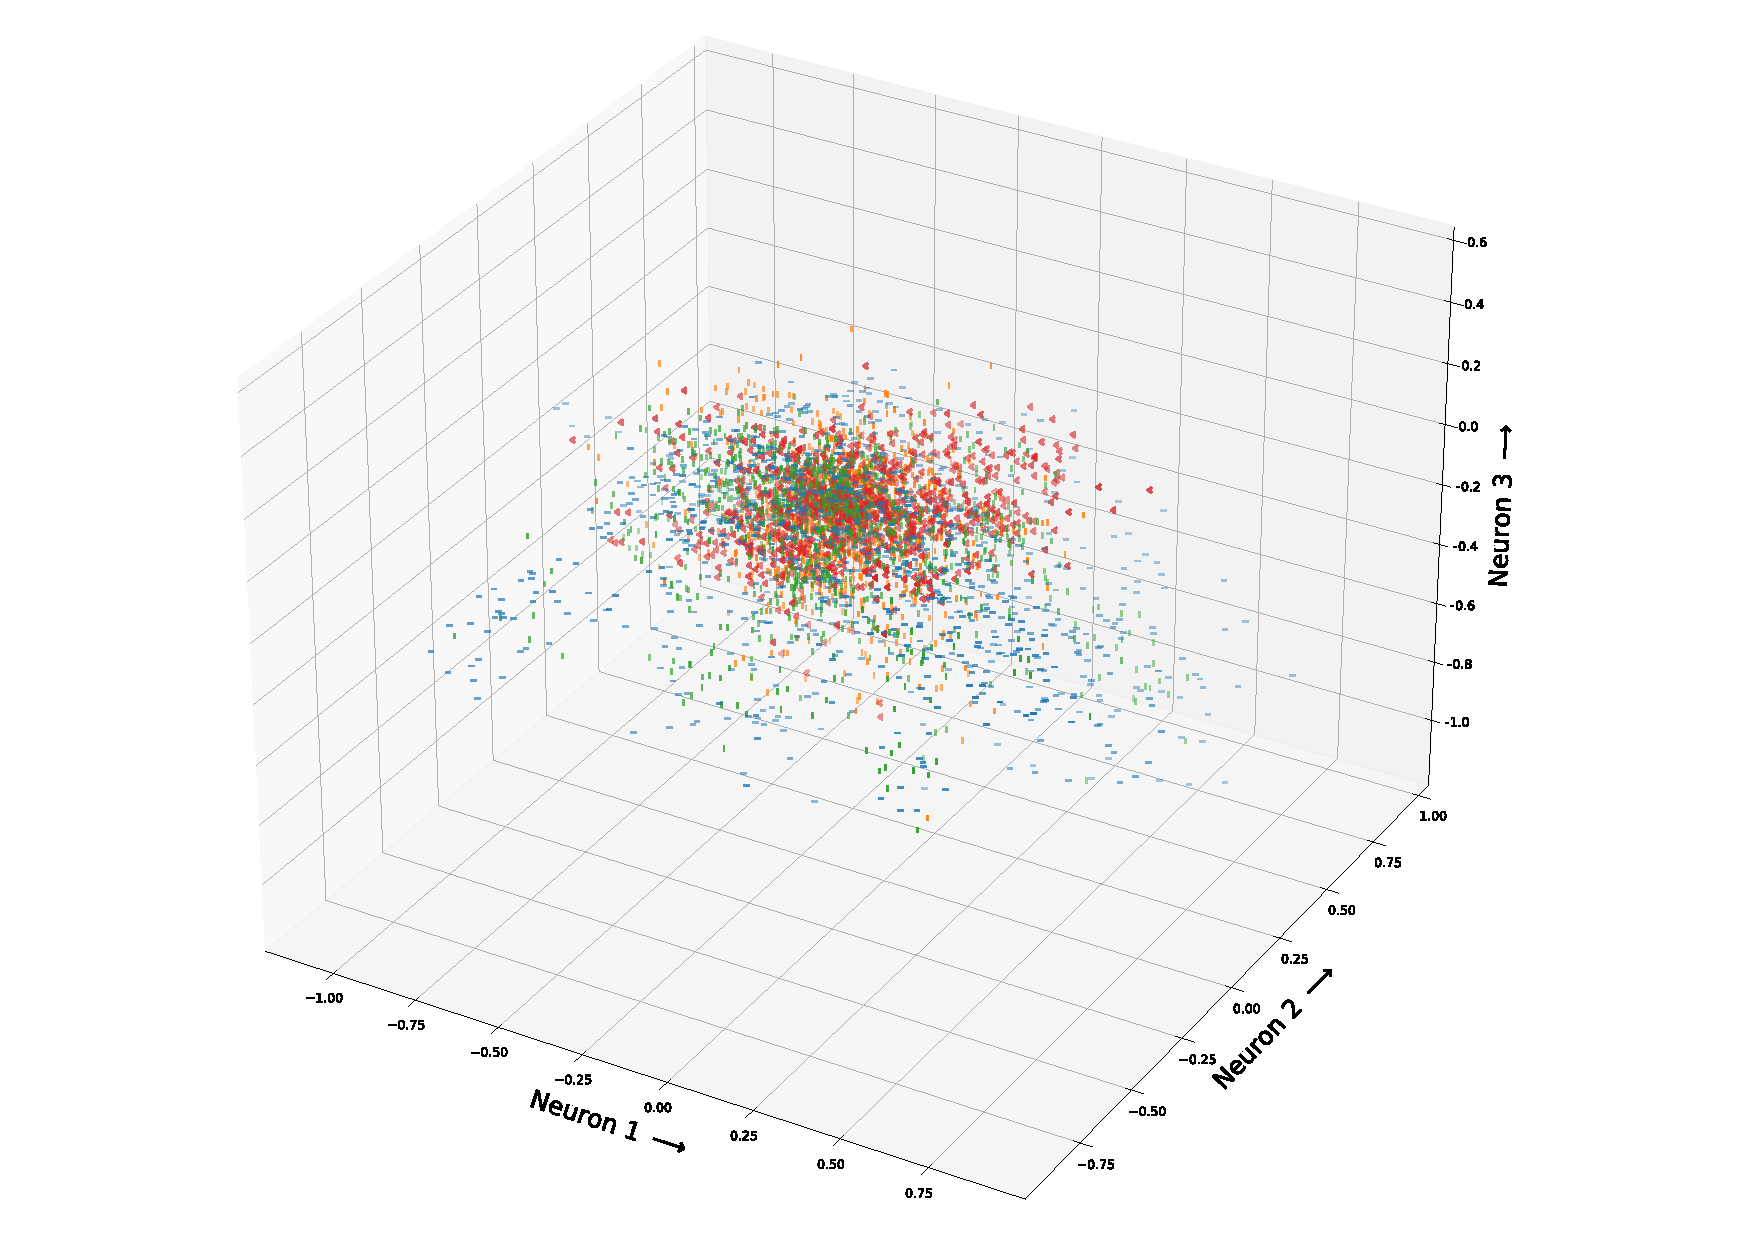
\includegraphics[width=.44\textwidth]{GAMMA_distribution/mmd_epoch0_0_1.pdf}
  \hspace{.3cm}
  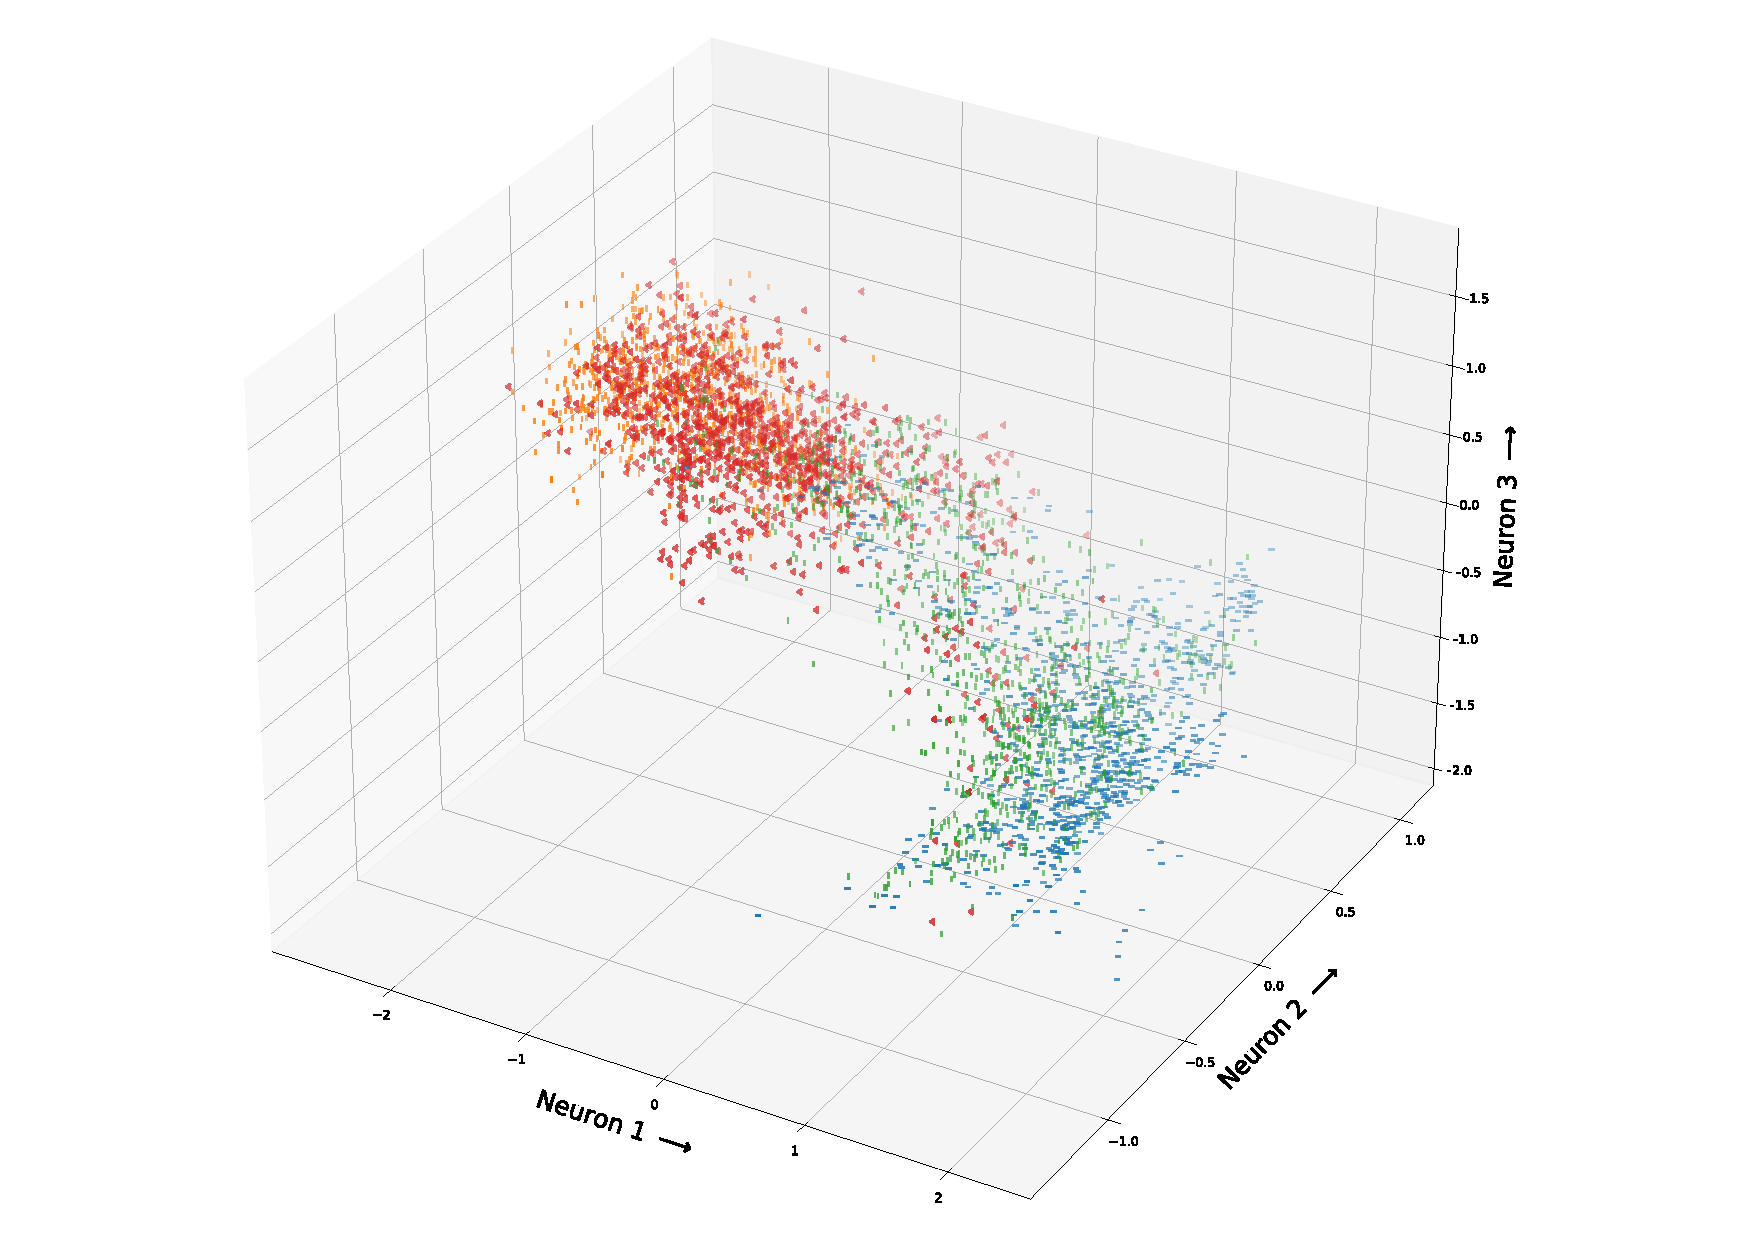
\includegraphics[width=.44\textwidth]{GAMMA_distribution/mmd_epoch8_0_1.pdf}

  \vspace{.1cm}

  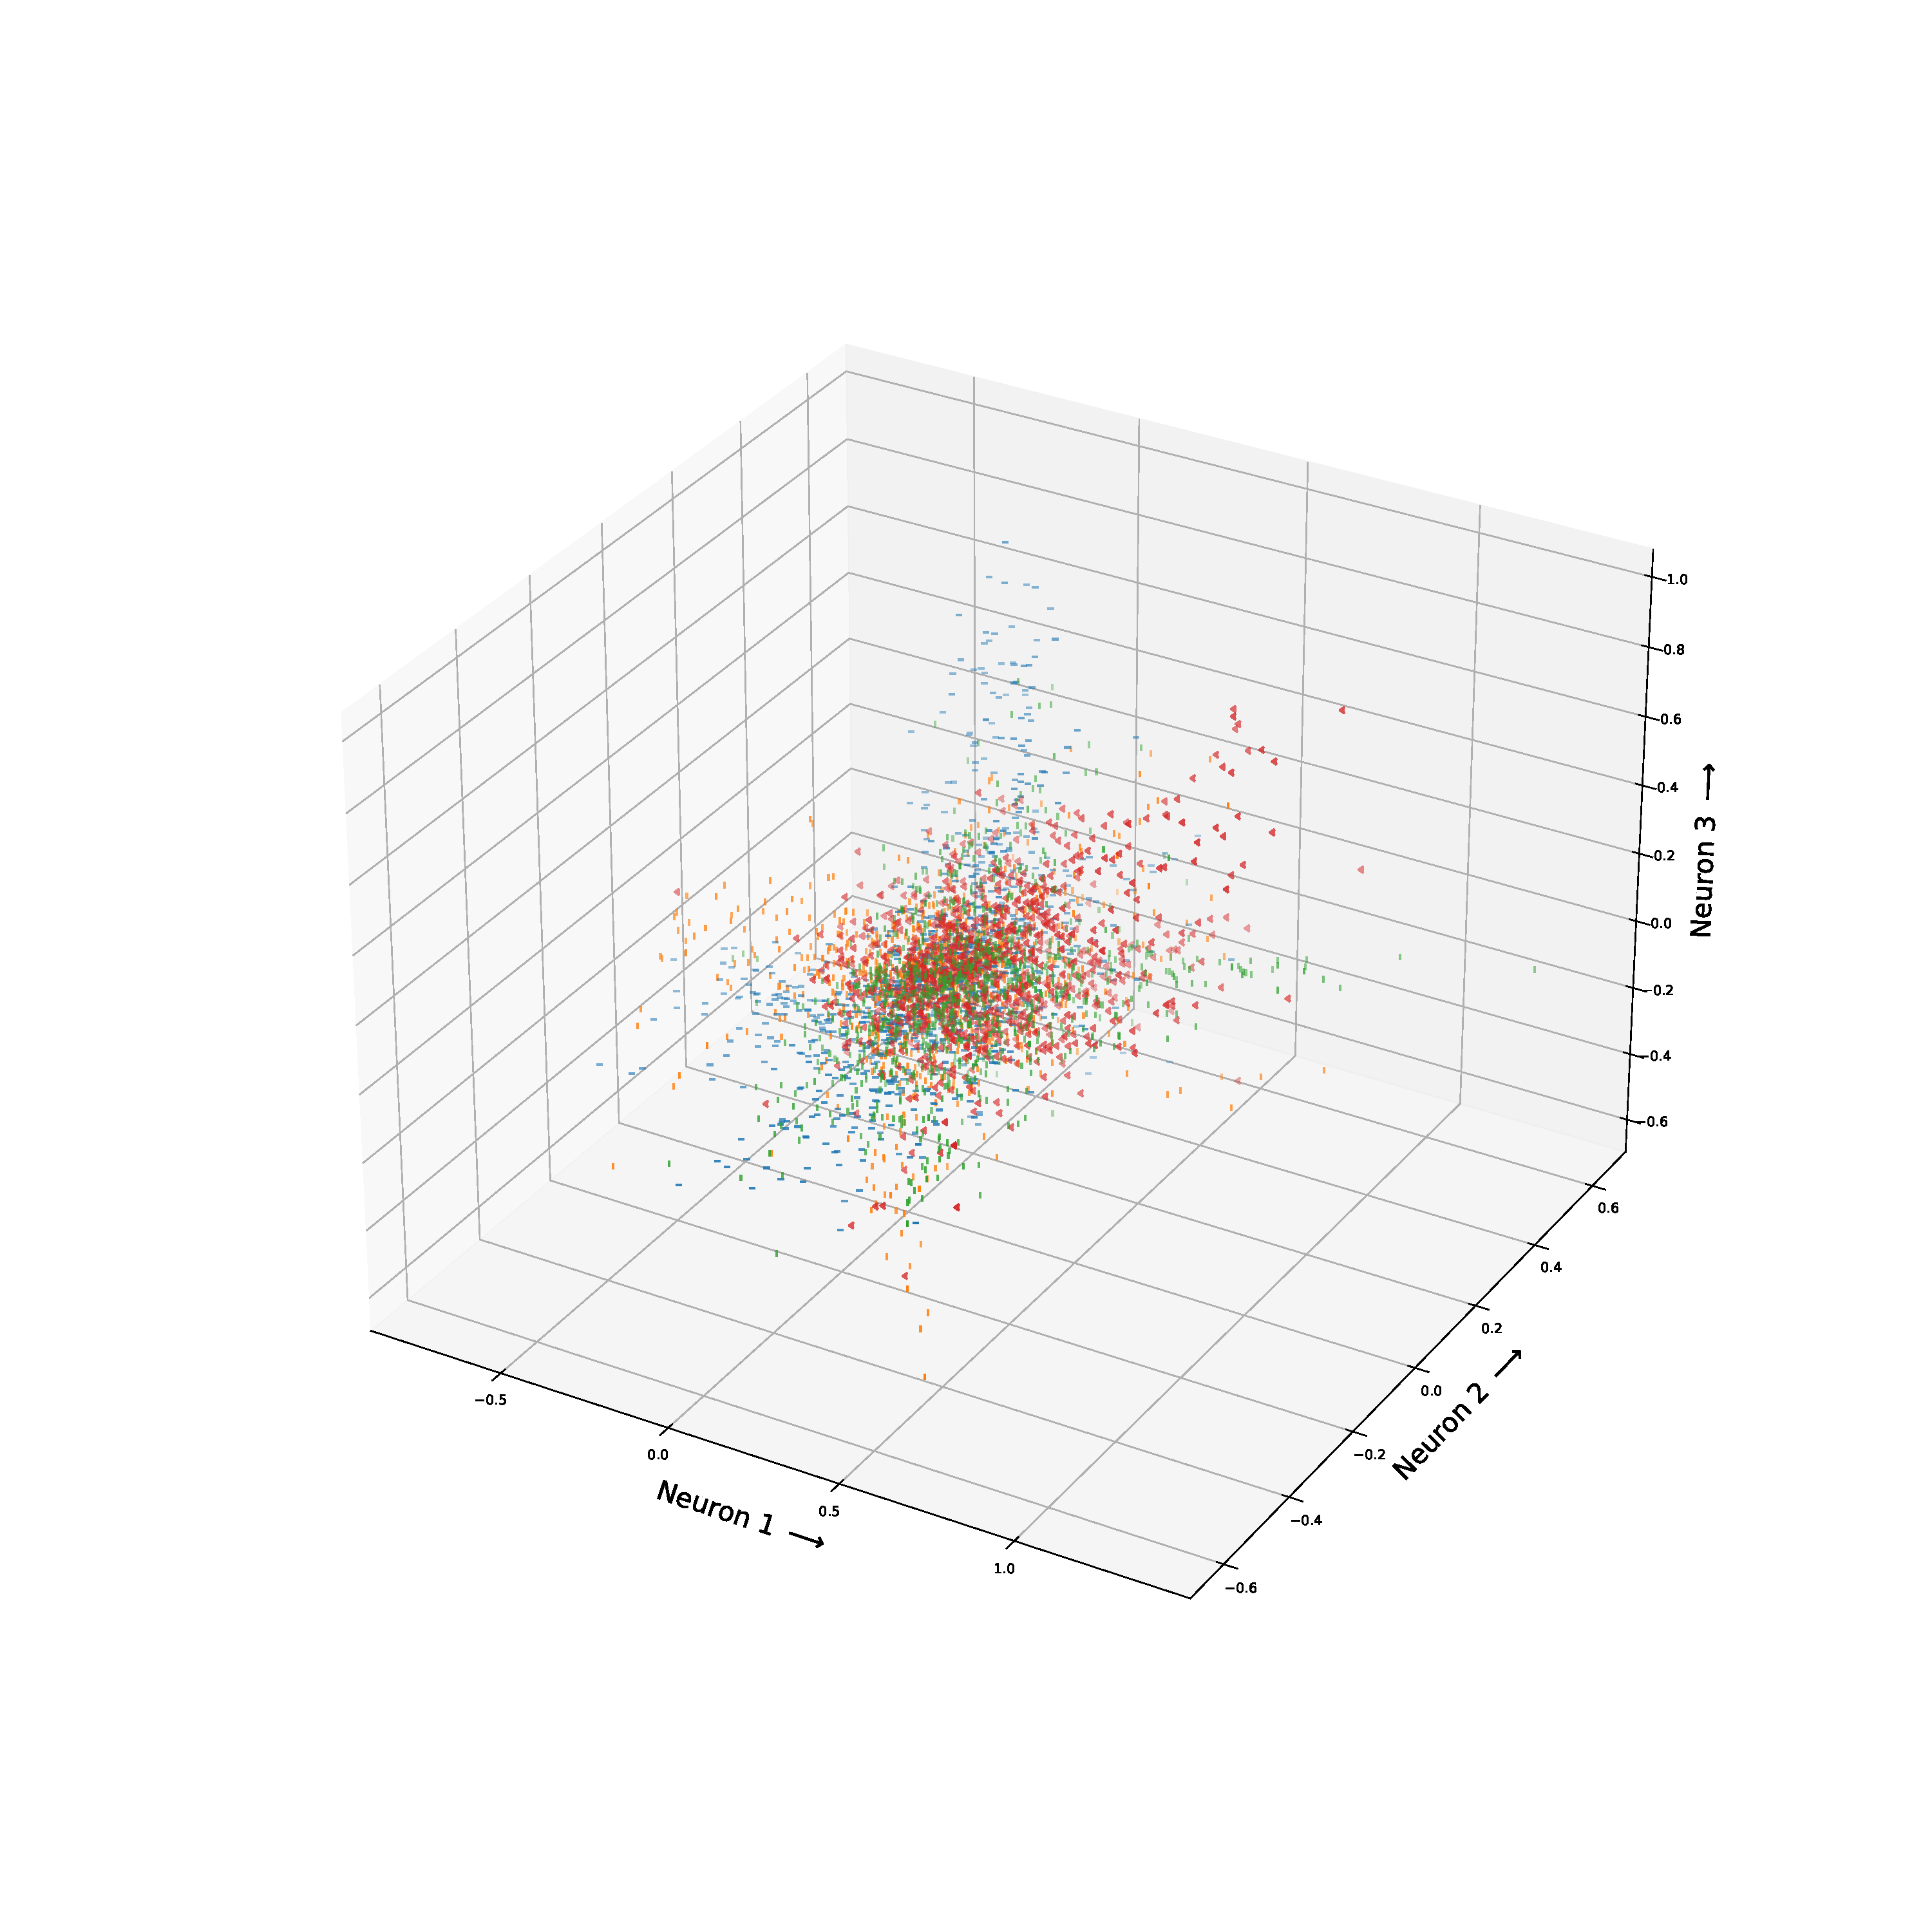
\includegraphics[width=.44\textwidth]{GAMMA_distribution/mmd_epoch0_0_5.pdf}
  \hspace{.3cm}
  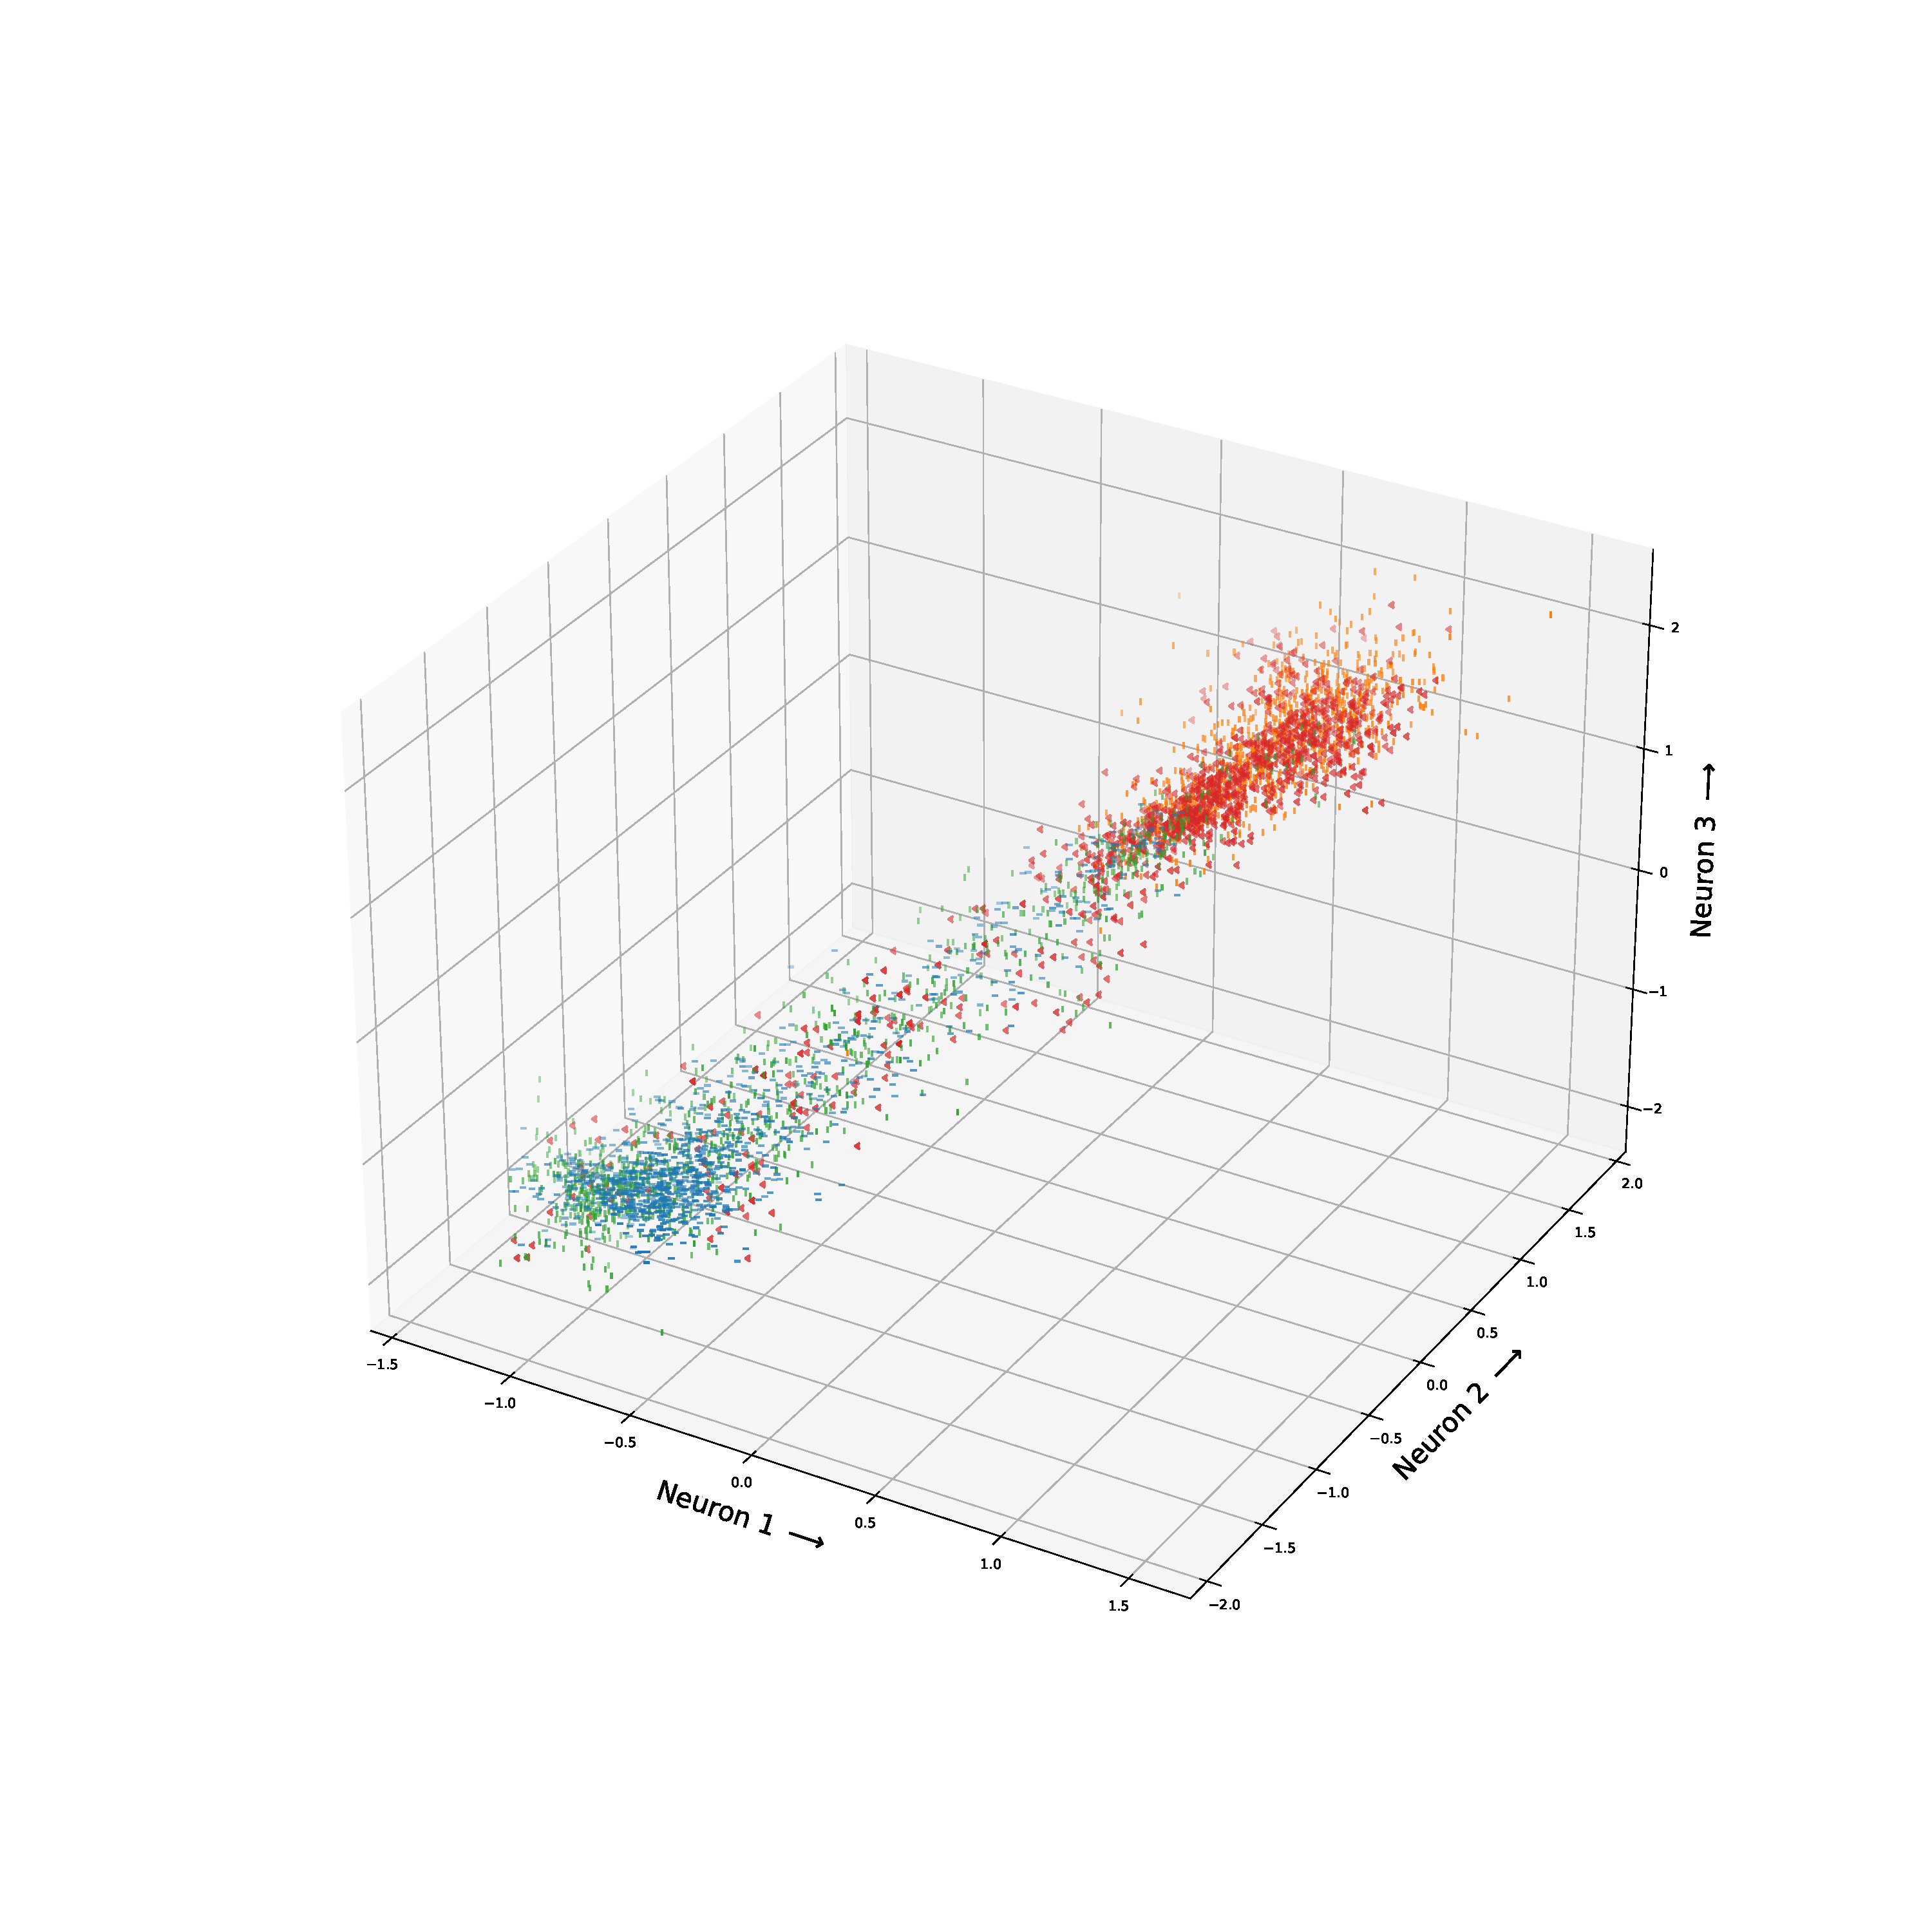
\includegraphics[width=.44\textwidth]{GAMMA_distribution/mmd_epoch8_0_5.pdf}

  \vspace{.1cm}

  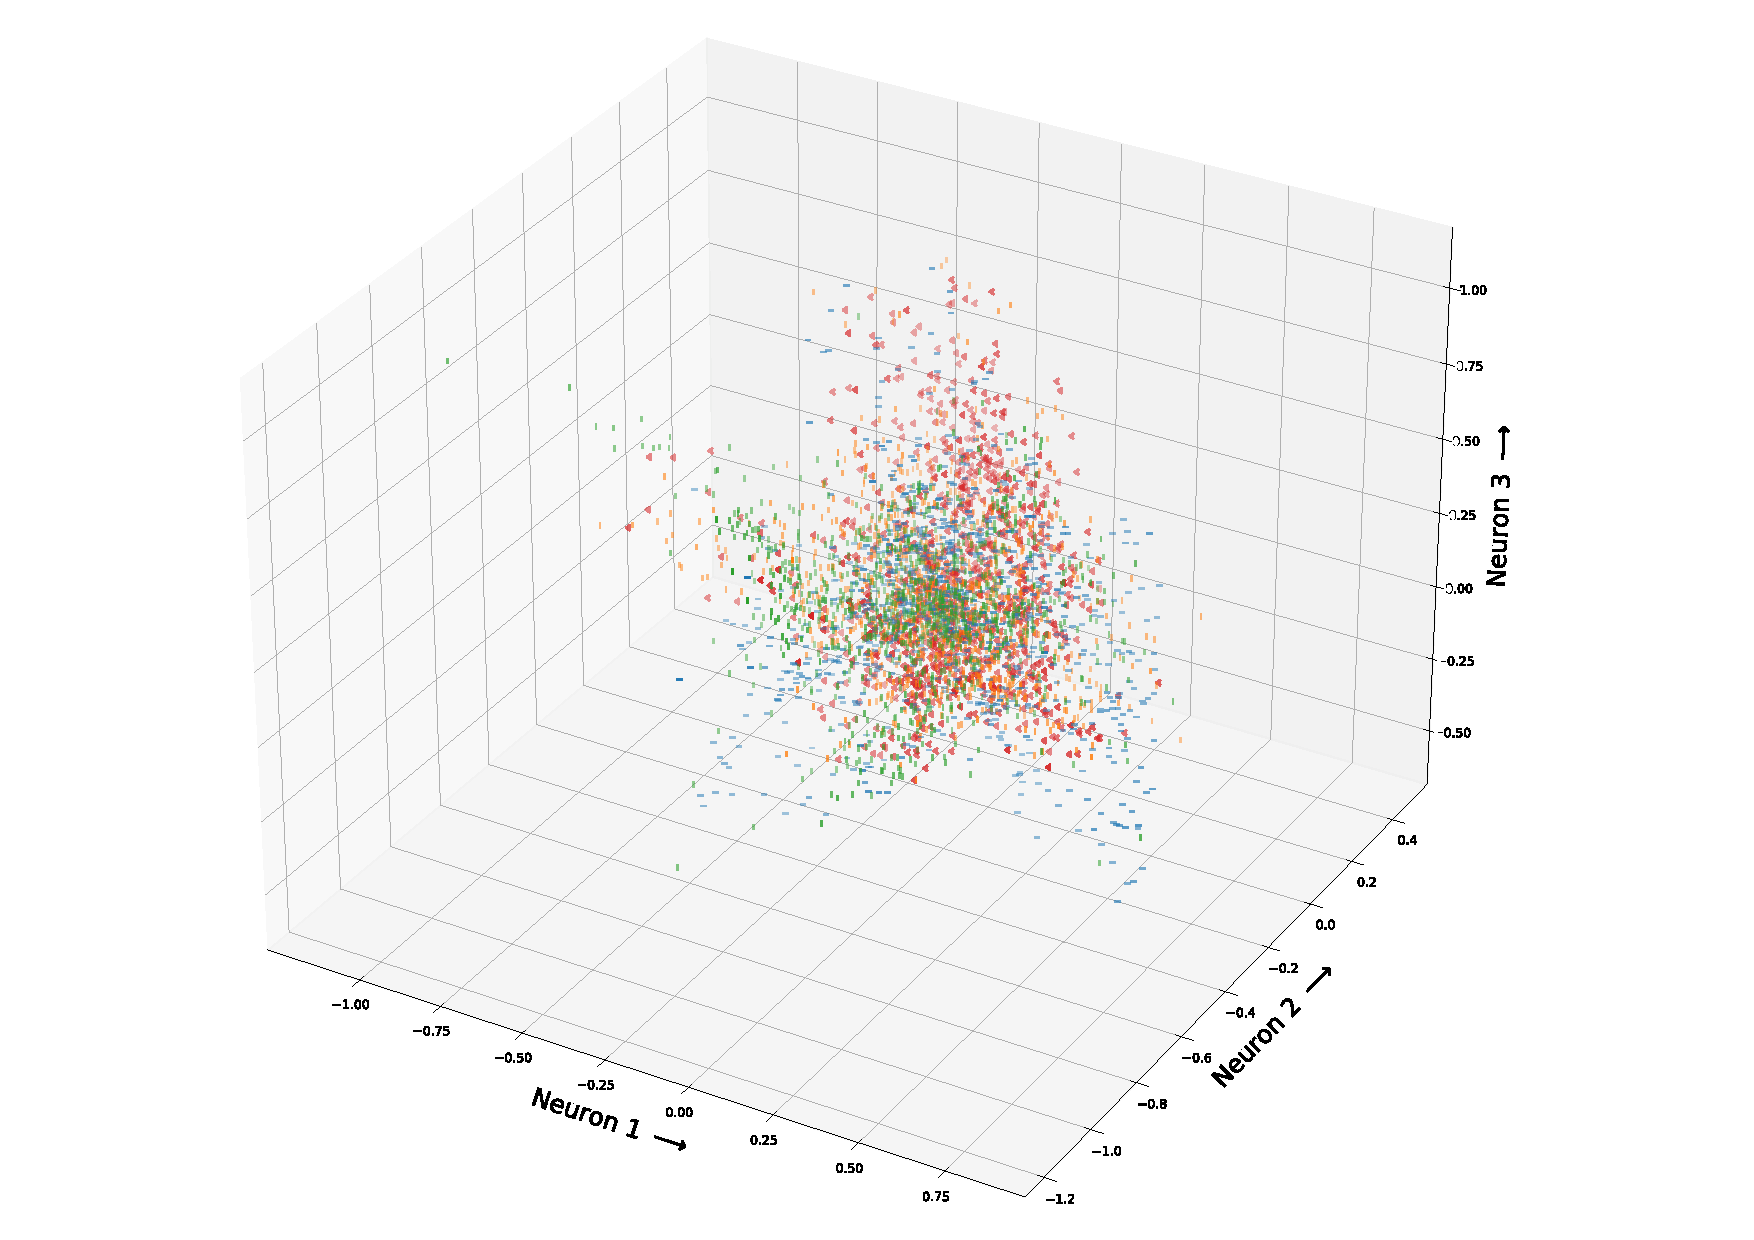
\includegraphics[width=.44\textwidth]{GAMMA_distribution/mmd_epoch0_30.pdf}
  \hspace{.3cm}
  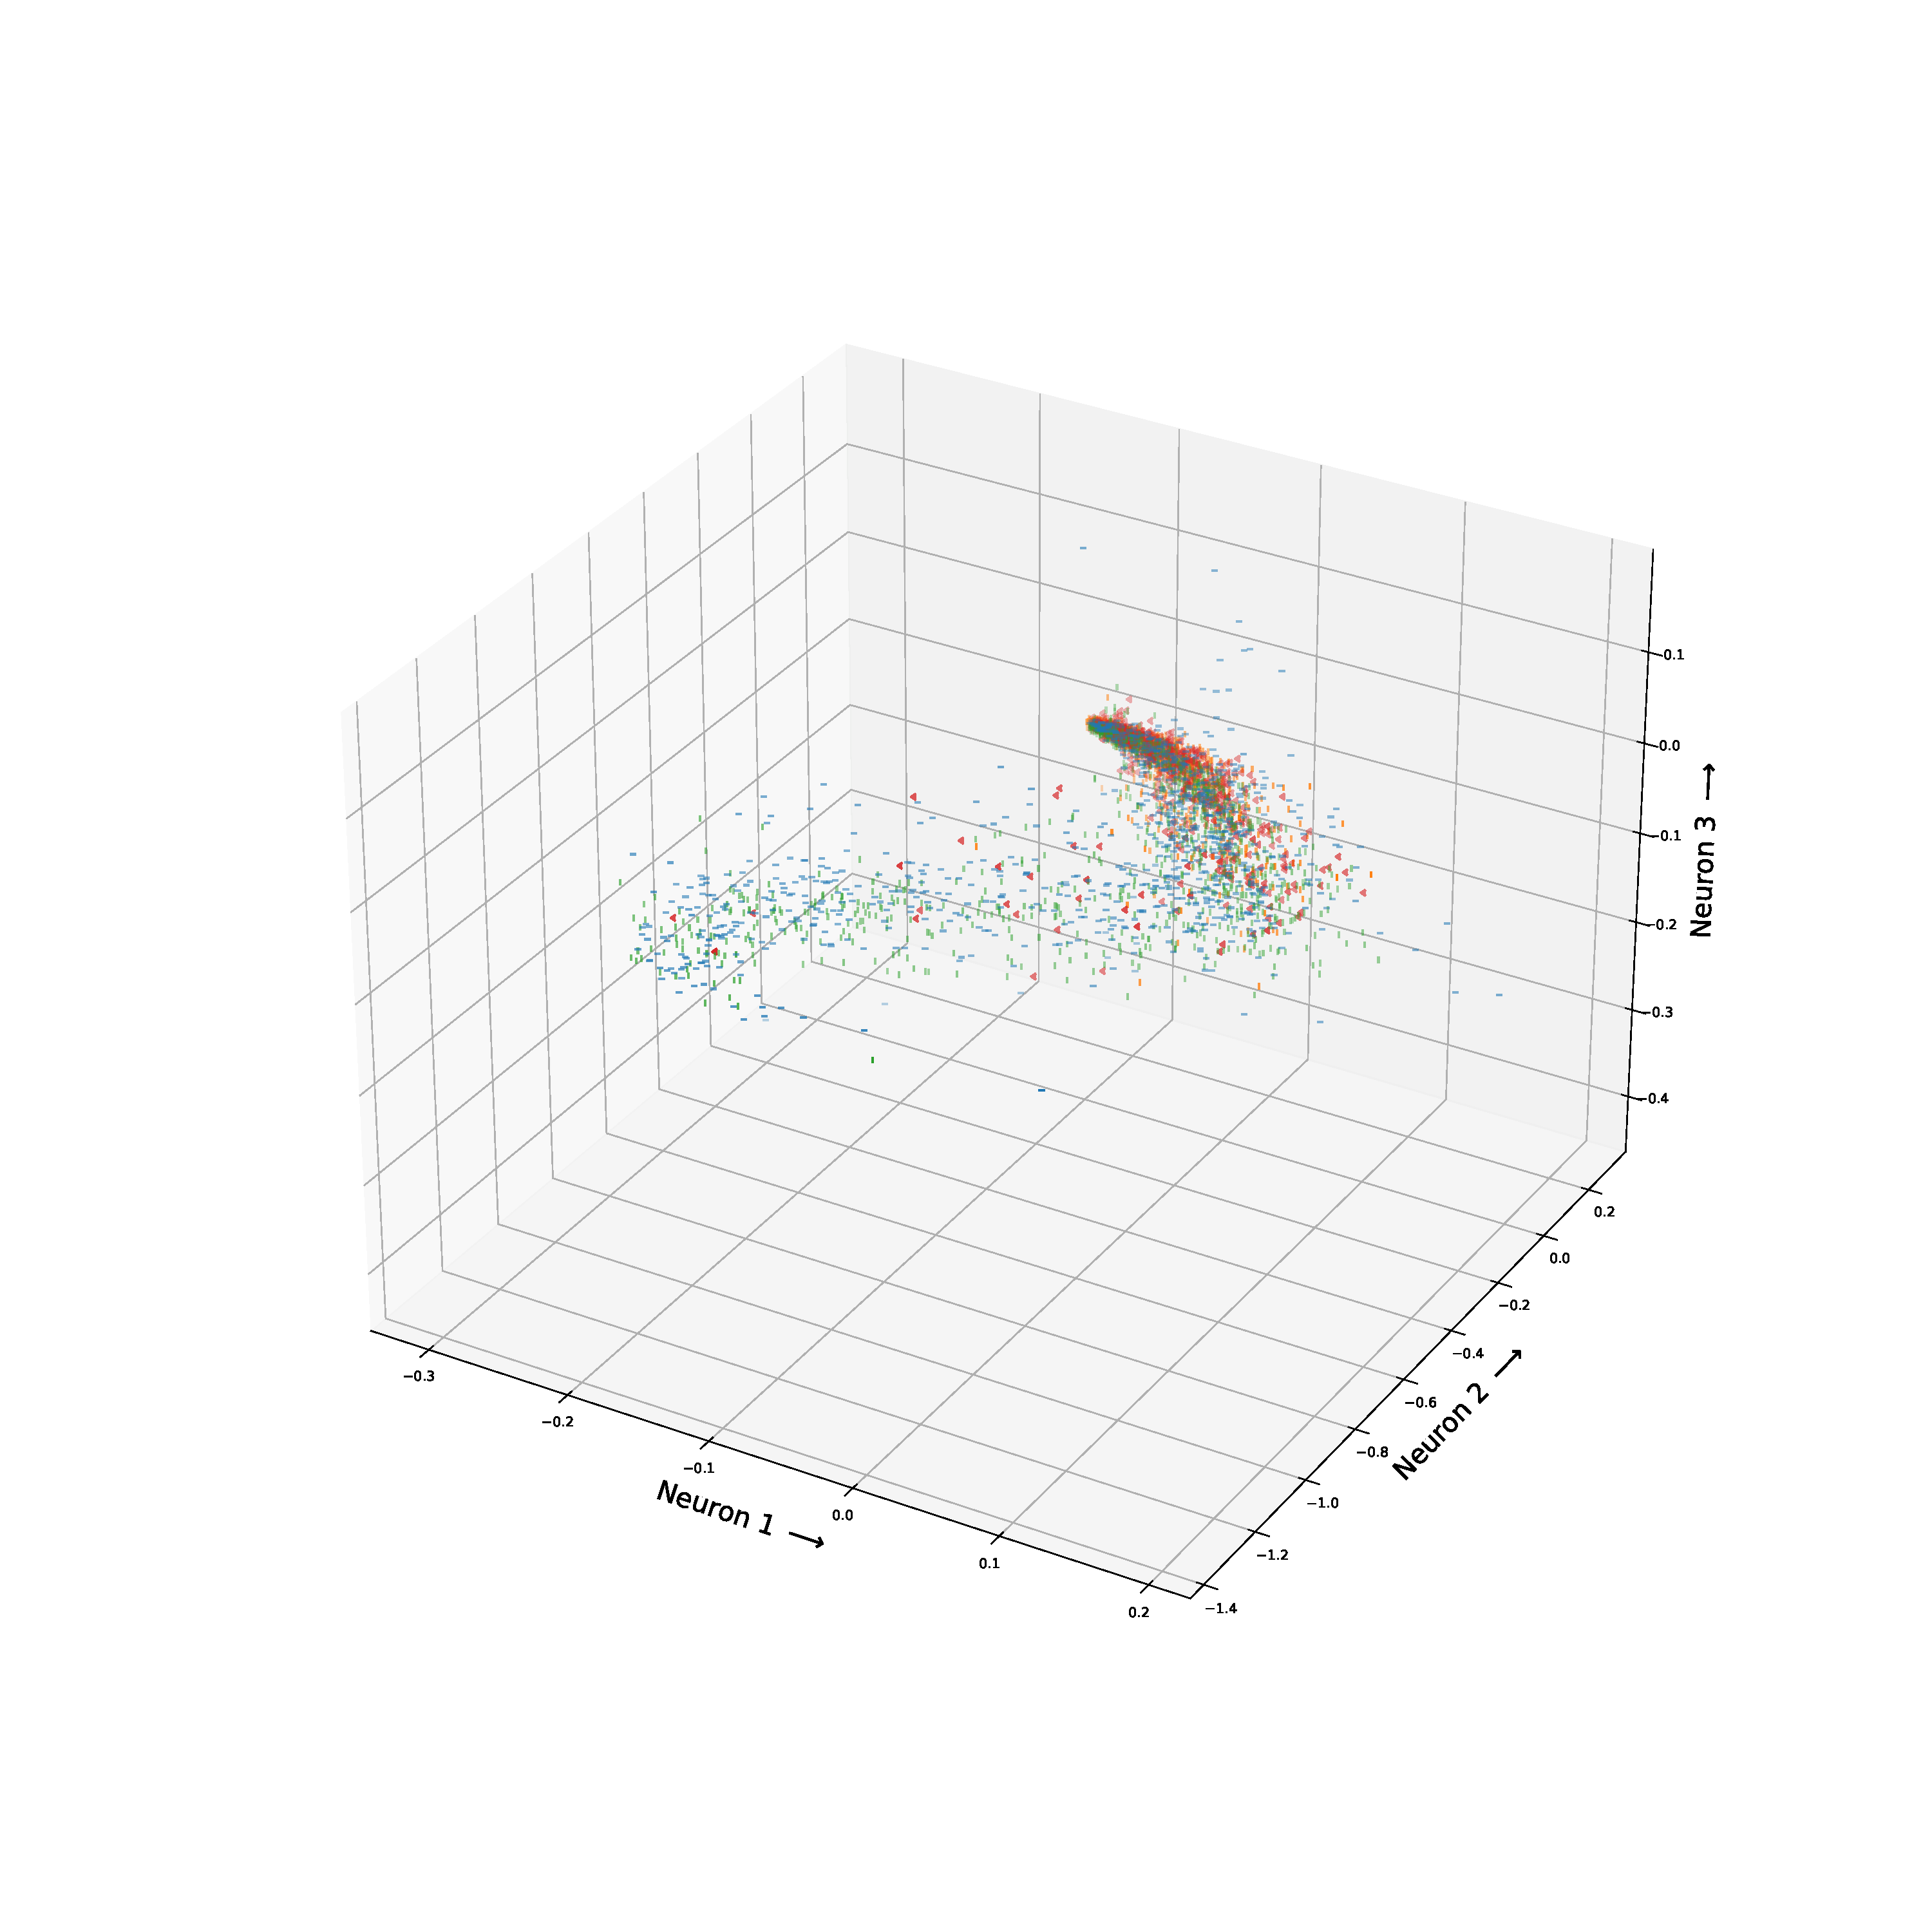
\includegraphics[width=.44\textwidth]{GAMMA_distribution/mmd_epoch8_30.pdf}
  
  \vspace{.1cm}
  
  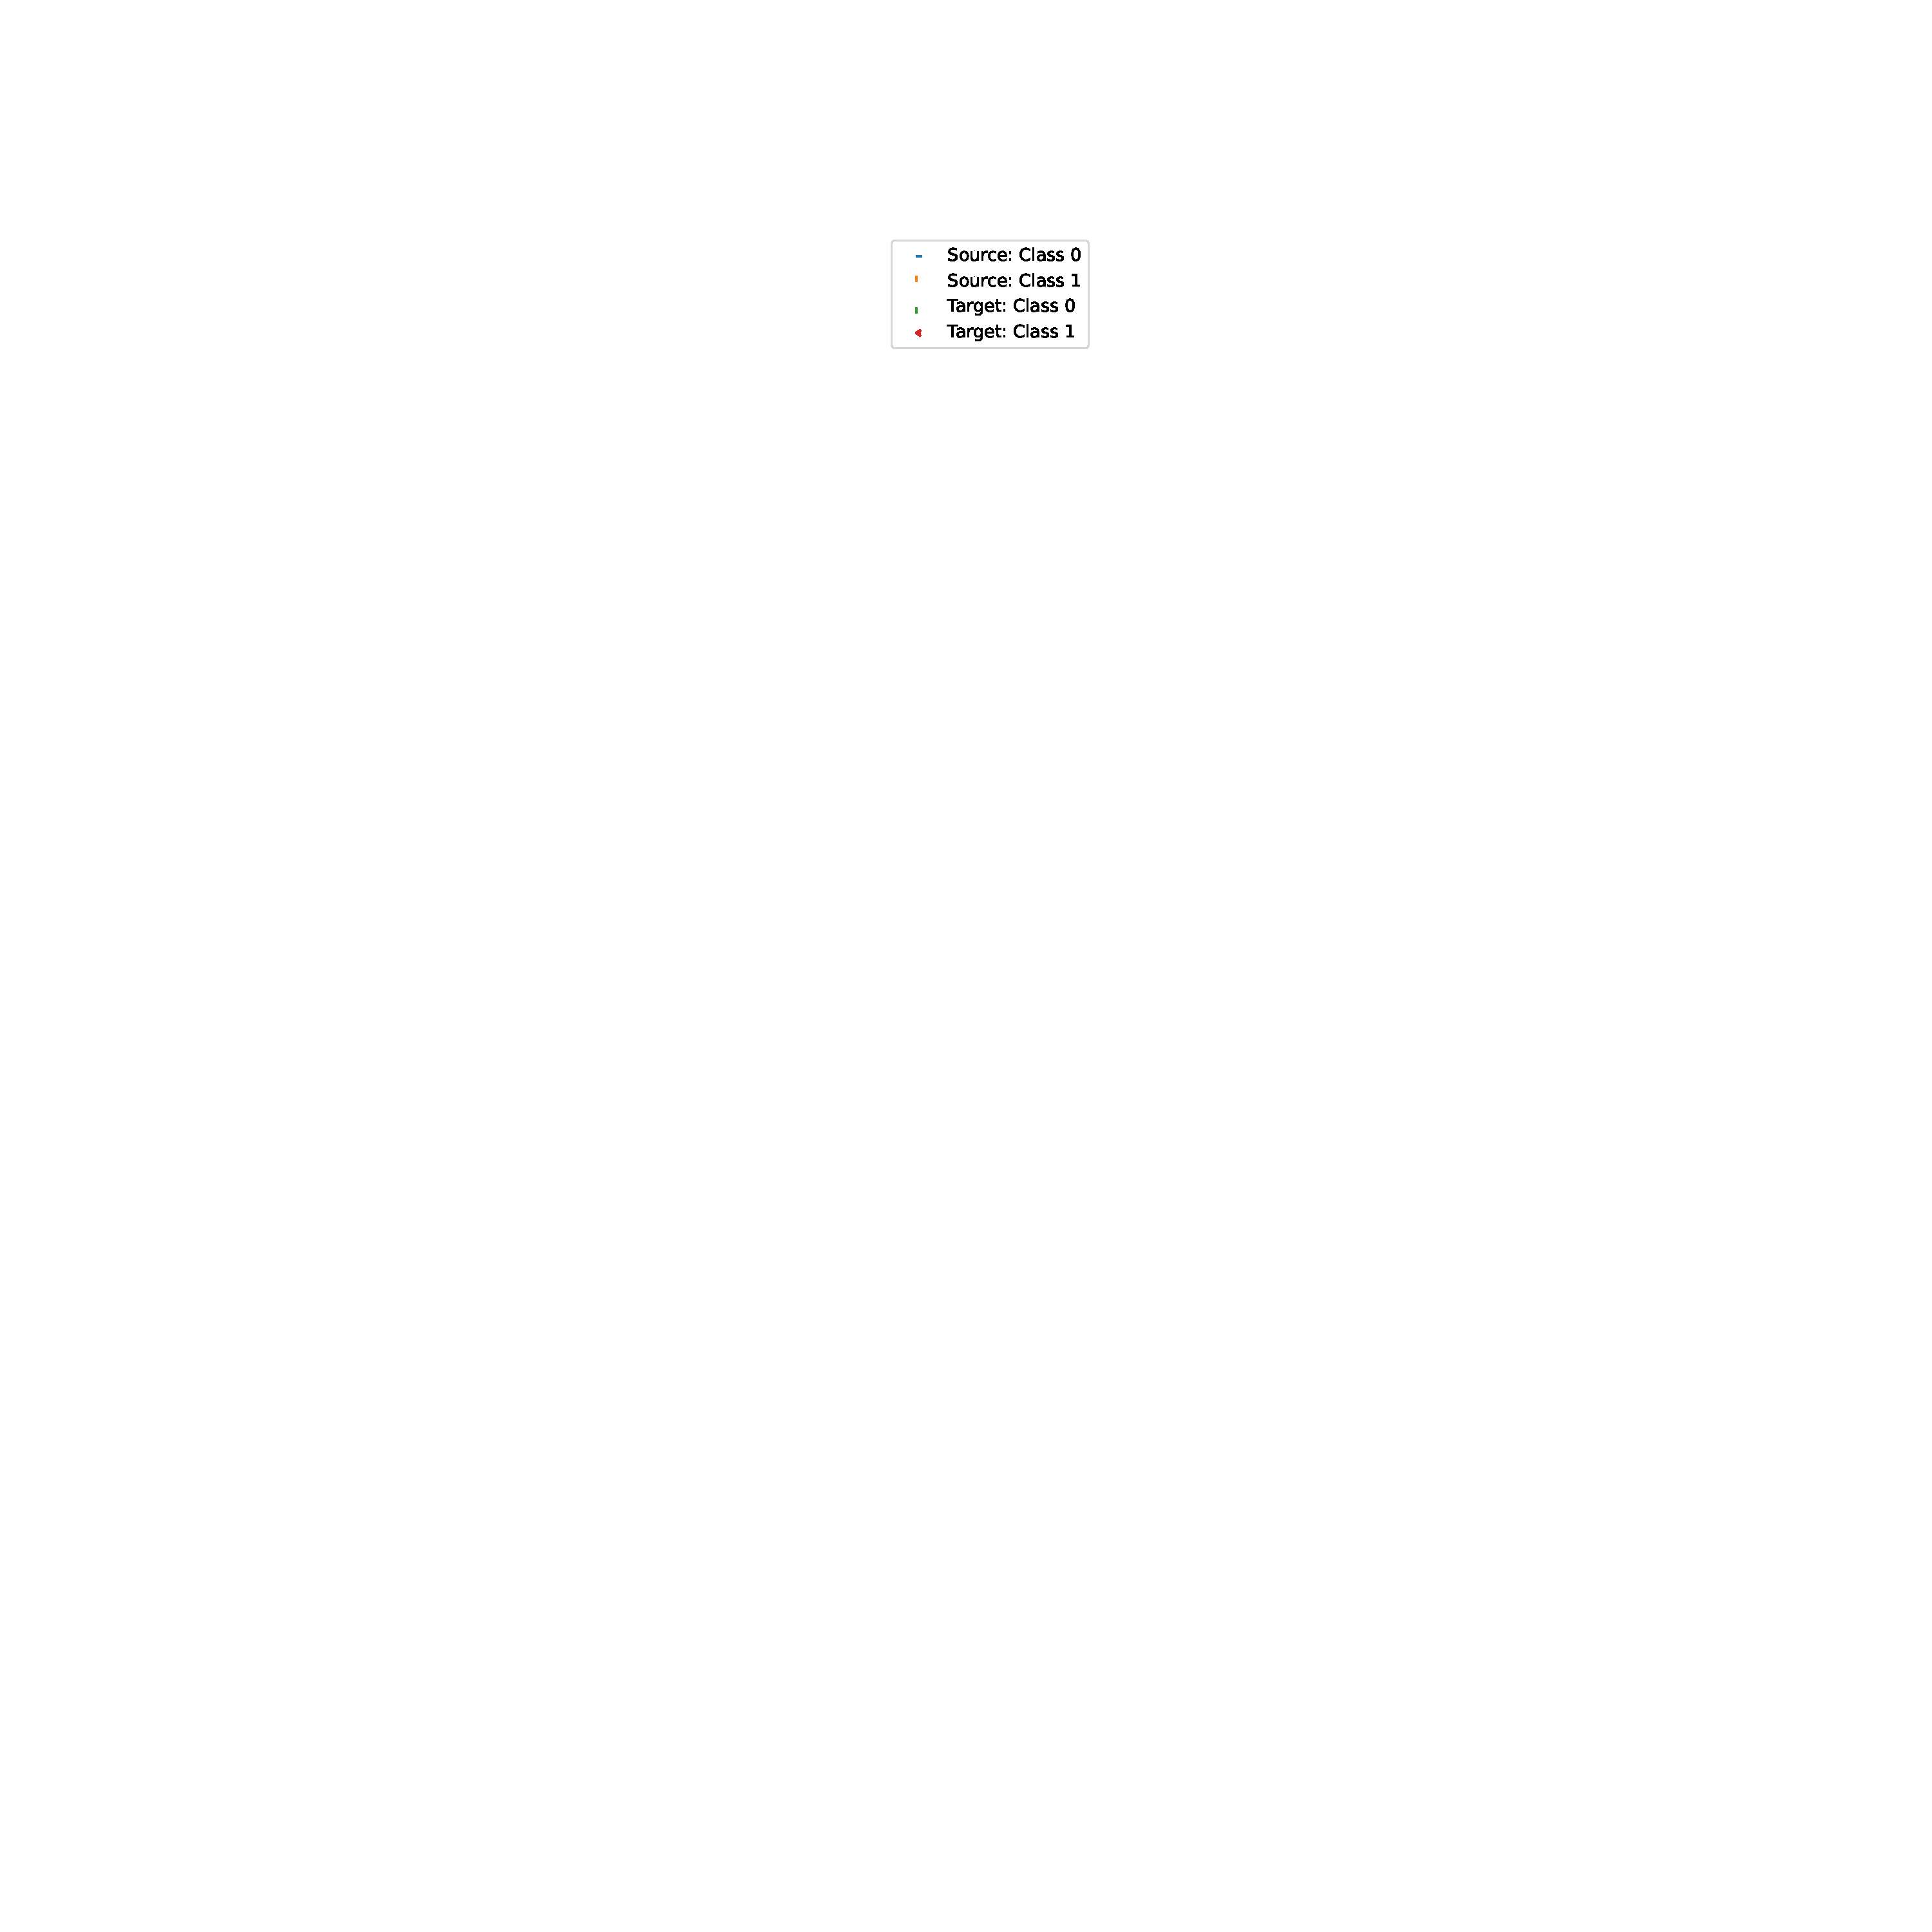
\includegraphics[width=.15\textwidth]{labeled_vs_unlabeled_point_cloud/legend.pdf}


  \caption{Data distribution: Influence of GAMMA on model training, with GAMMA = 0.1 (top), GAMMA = 0,5 (middle), GAMMA = 30 (bottom)}
  \label{fig:point_cloud_mmd}
\end{figure}





\begin{figure}[H]
  \centering
  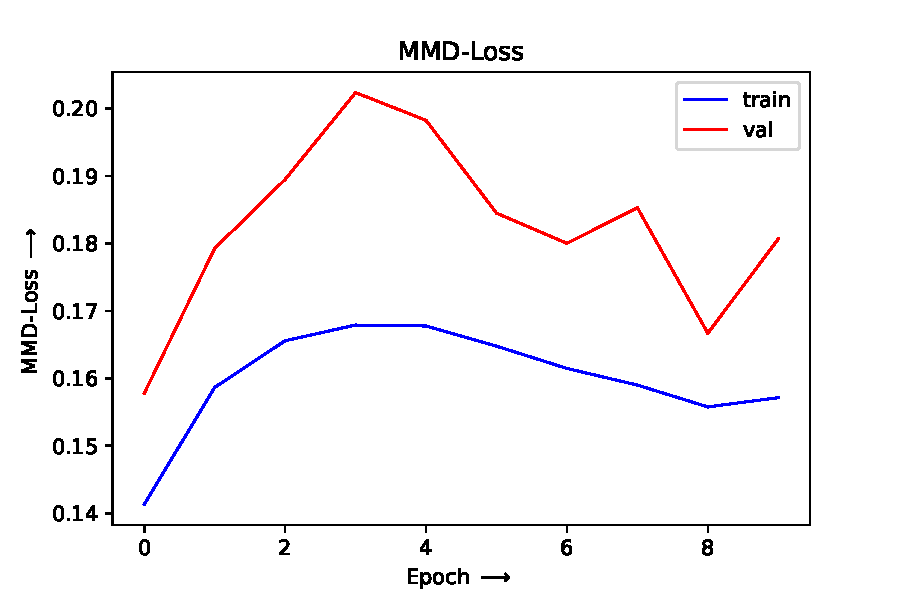
\includegraphics[width=.45\textwidth]{GAMMA_plot/mmd_loss_0_1.pdf}
  \hspace{.3cm}
  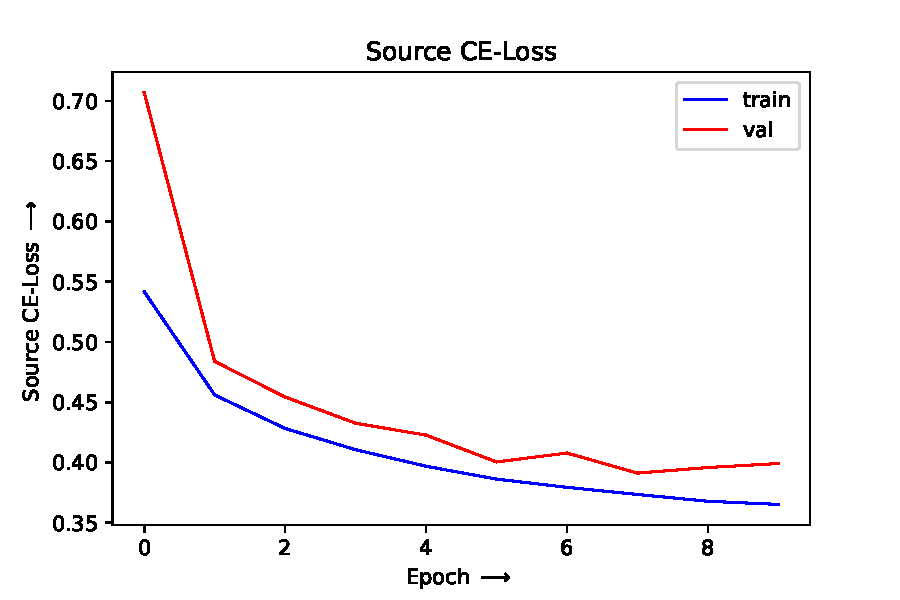
\includegraphics[width=.45\textwidth]{GAMMA_plot/source_ce_loss_0_1.pdf}

  \vspace{.3cm}

  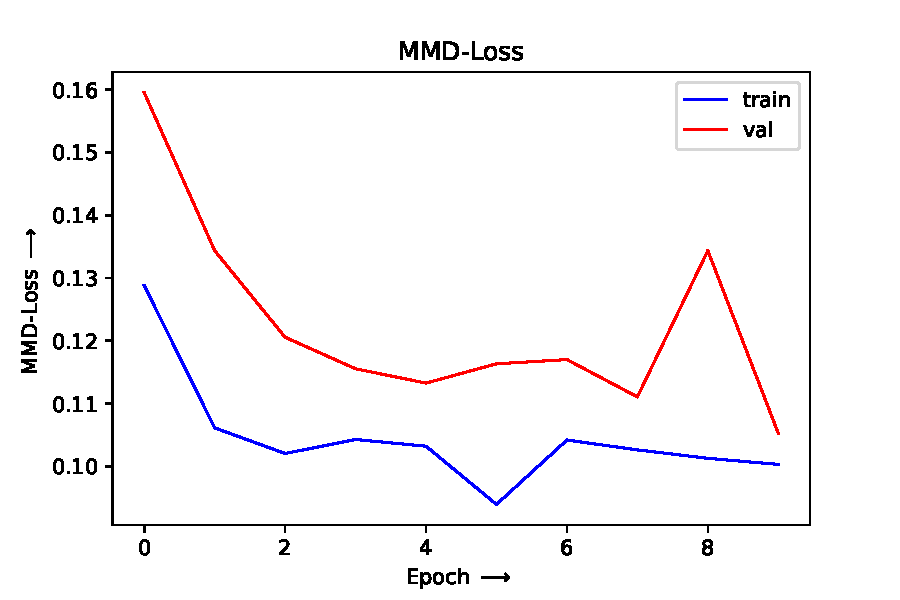
\includegraphics[width=.45\textwidth]{GAMMA_plot/mmd_loss_0_5.pdf}
  \hspace{.3cm}
  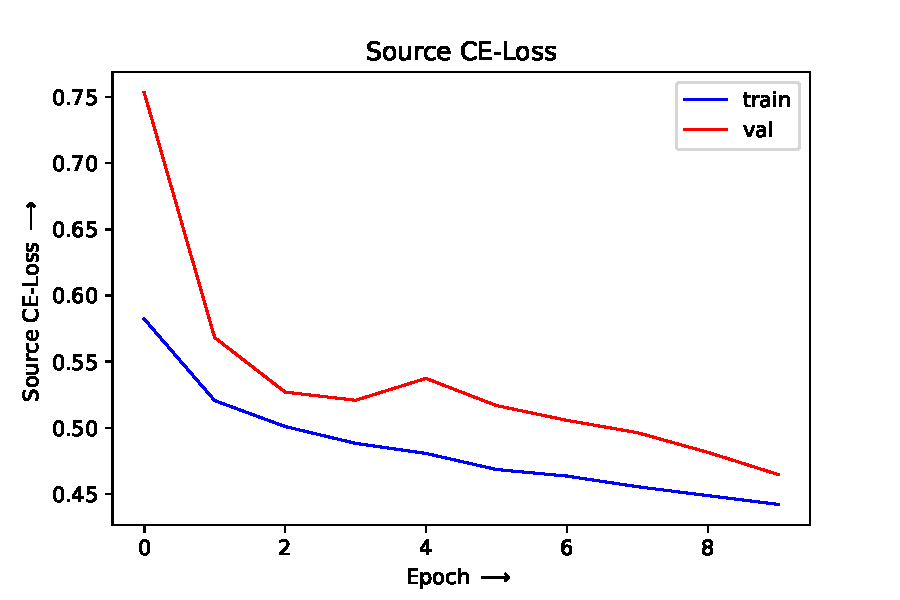
\includegraphics[width=.45\textwidth]{GAMMA_plot/source_ce_loss_0_5.pdf}

  \vspace{.3cm}

  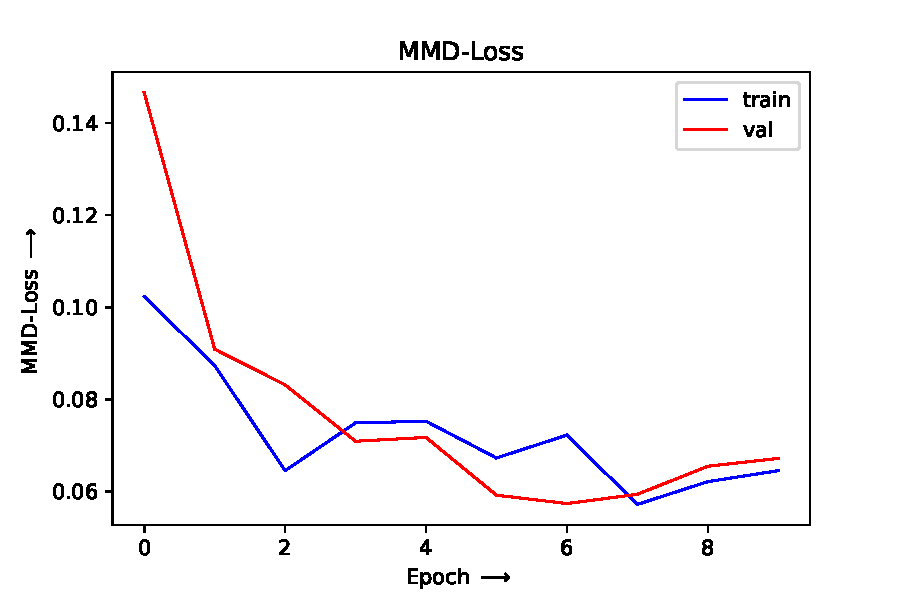
\includegraphics[width=.45\textwidth]{GAMMA_plot/mmd_loss_30.pdf}
  \hspace{.3cm}
  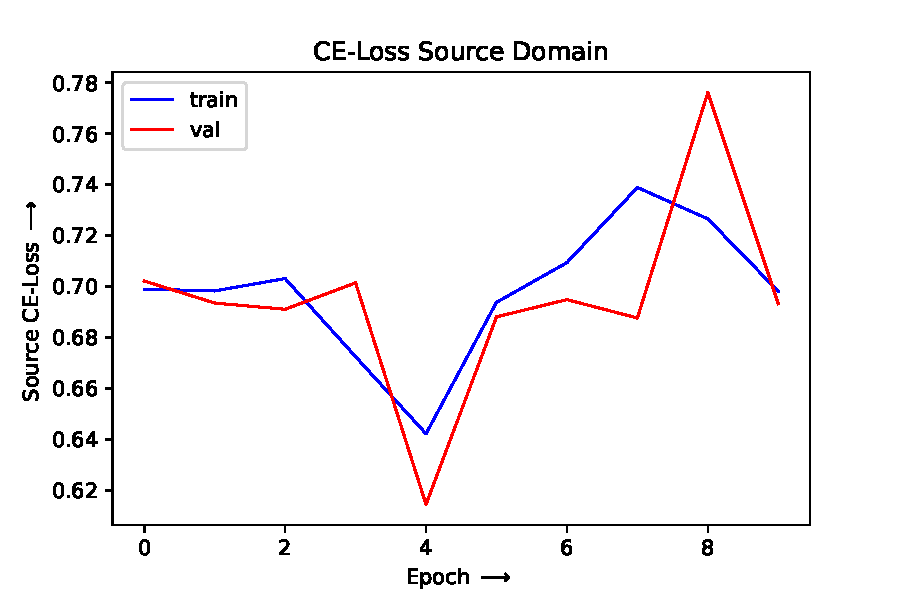
\includegraphics[width=.45\textwidth]{GAMMA_plot/source_ce_loss_30.pdf}

  \caption{MMD and Source CE-Loss curves: Influence of GAMMA on model training, with GAMMA = 0.1 (top), GAMMA = 0,5 (middle), GAMMA = 30 (bottom)}
  \label{fig:learning_curves_influence_mmd_feature_extractor}
\end{figure}

\subsection{Labeled vs. unlabeled MMD loss} \label{sec:Differences of labeled and unlabeled MMD loss}

The idea behind domain adaption is to aggregate knowledge while solving one problem and transferring that knowledge to another problem. For this reason, in domain adaption tasks the goal is to restrict the supervised learning solely on the source domain data. In the regular MMD loss, the target labels are unknown. Therefore, the intra- and inter-class distance between source and target samples is minimized equally. Obviously, this reduces the class separability in both domains. In the literature, domain adaption approaches which use a small amount of the target domain labels are known as "Few-shot transfer learning" \cite{WU2020}. Similarly, in this section the effect of including a few target labels into the training is analyzed. The cross-entropy loss is still restricted to the source domain. Solely the MMD loss is allowed to use target labels. The distance between source and target samples of similar and different classes can be calculated separately. The labeled MMD loss optimizes the model such, that the intra-class distance is maximized and the inter-class distance is minimized for both domains. This separate consideration of class distances allows a simultaneous improvement of class separability and compactness. Besides that, the training includes the source cross-entropy loss. The hyperparameters GAMMAIntraClass and GAMMAInterClass are used to balance the training scope of minimizing the inter-, maximizing the intra-class distance and increasing the source domain classification performance:

\begin{equation}
\begin{split}
    TotalMMDLoss = GAMMAIntraClass * MMDLossIntraClass\\ + GAMMAInterClass * MMDLossInterClass + CELoss
\end{split}
\end{equation}

 The MMD loss which includes the target labels is named "labeled MMD loss" and otherwise "unlabeled MMD loss". Again, fig. \ref{fig:point_cloud_labeled_unlabeled_mmd} visualizes the latent feature representation in FC2. Throughout the training, the labeled MMD loss is able to reduce the domain discrepancy while increasing the separability and compactness of the classes in both domains. This simplifies the classification problem and makes the model optimization less prone to find a trivial solution, in which the latent feature representation of all samples collapse at one point or a needle-like subspace. In this experiment, 20\% of target labels were used in labeled MMD loss.
\begin{figure}[H]
  \centering
  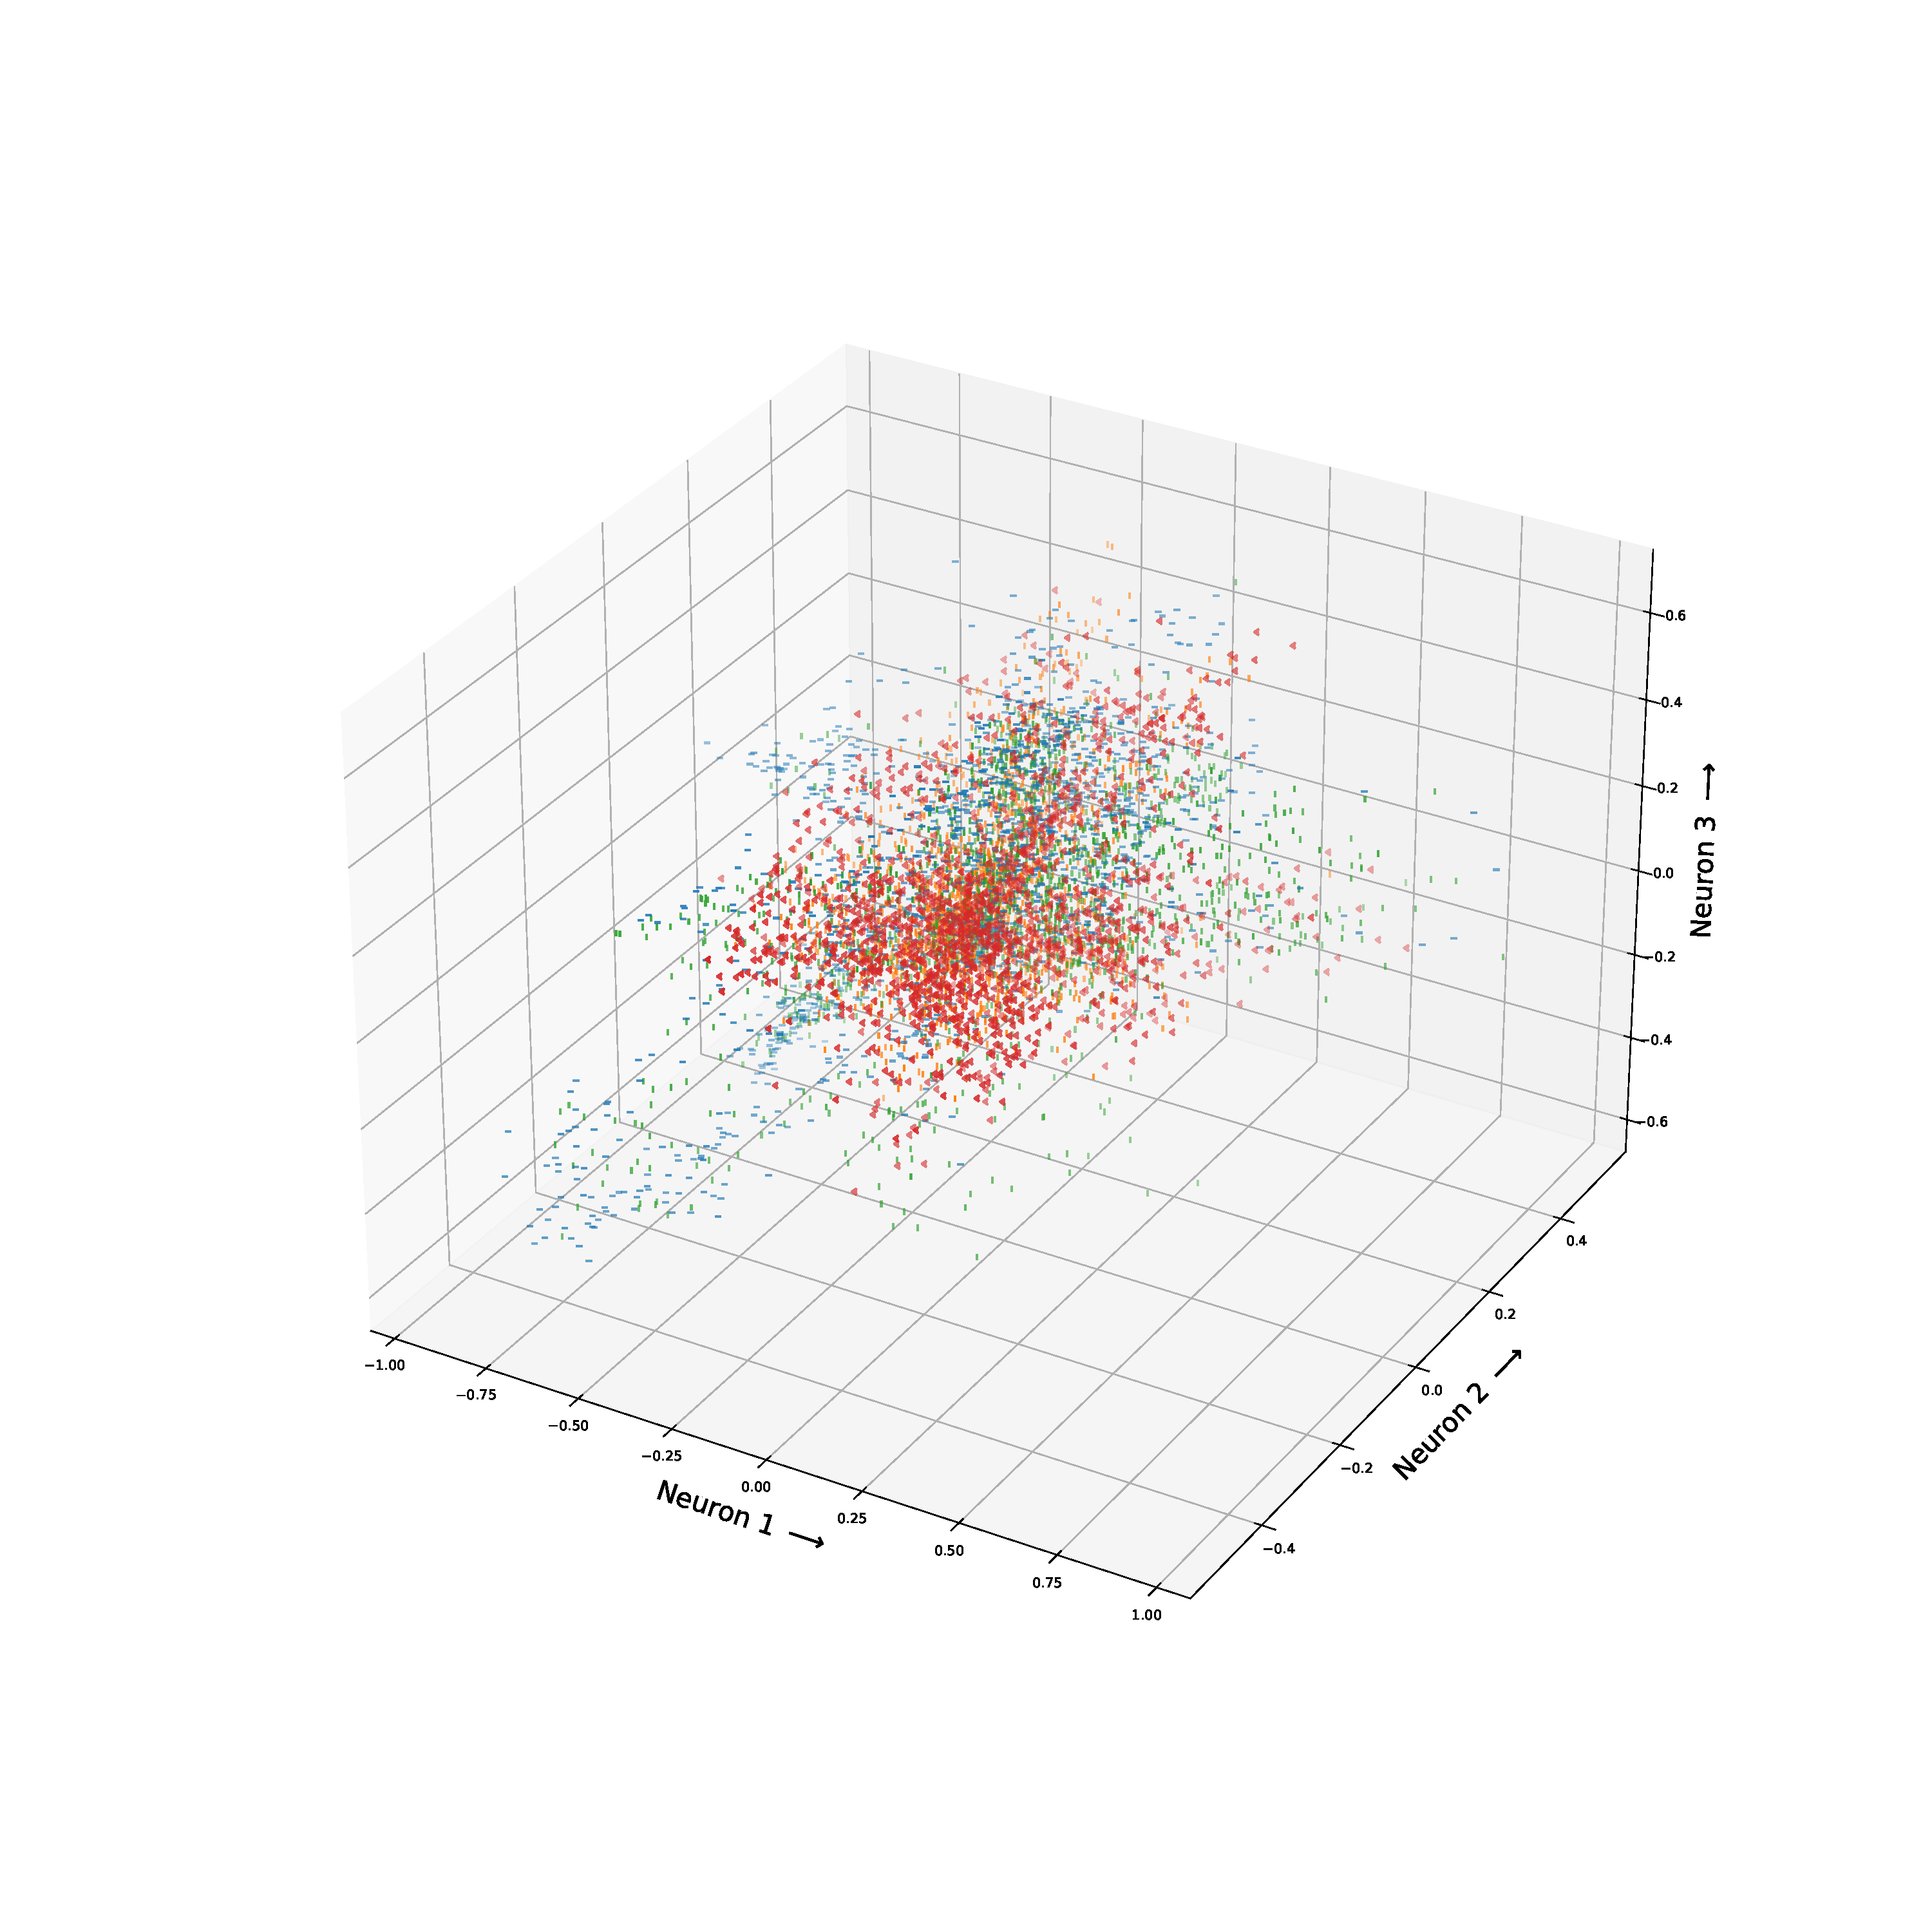
\includegraphics[width=.44\textwidth]{labeled_vs_unlabeled_point_cloud/labeled_mmd_epoch0.pdf}
  \hspace{.3cm}
  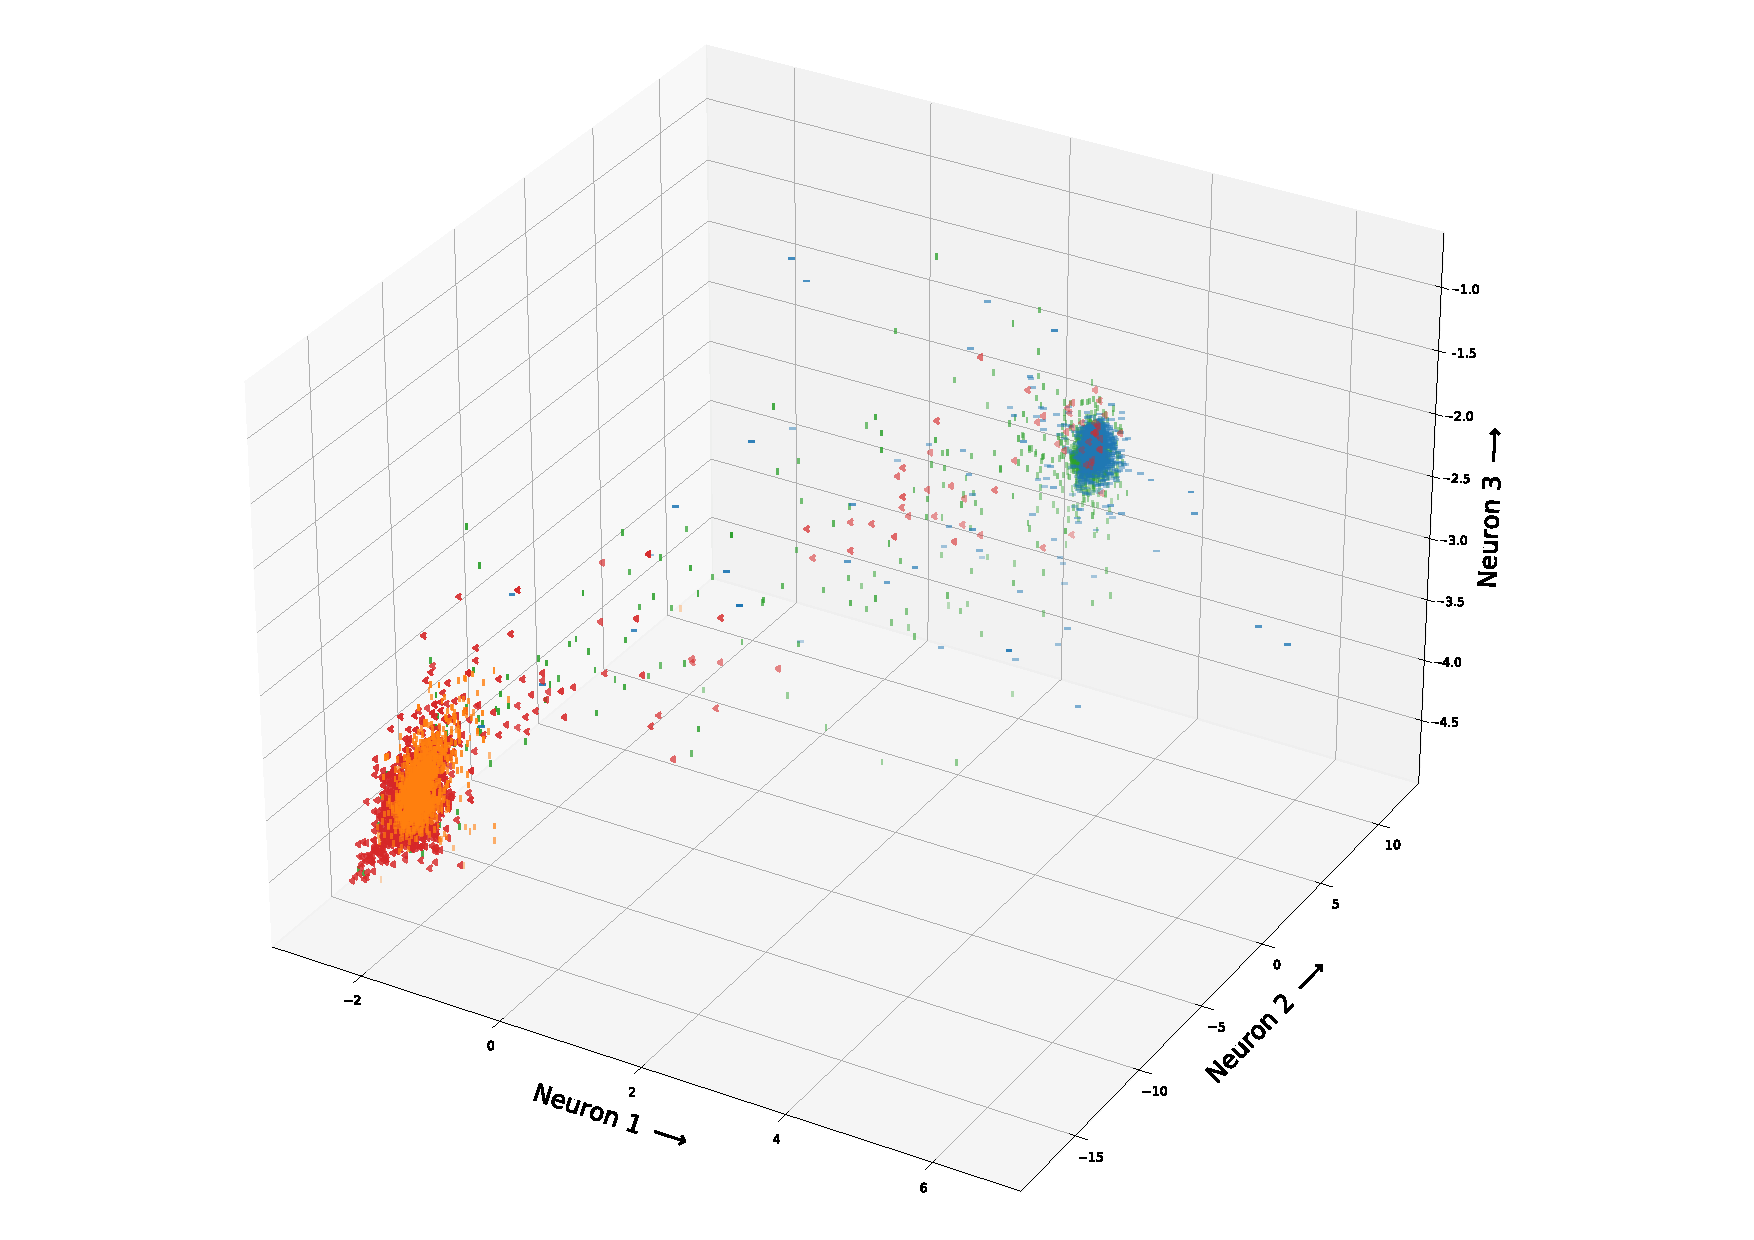
\includegraphics[width=.44\textwidth]{labeled_vs_unlabeled_point_cloud/labeled_mmd_epoch6.pdf}

  \vspace{.1cm}

  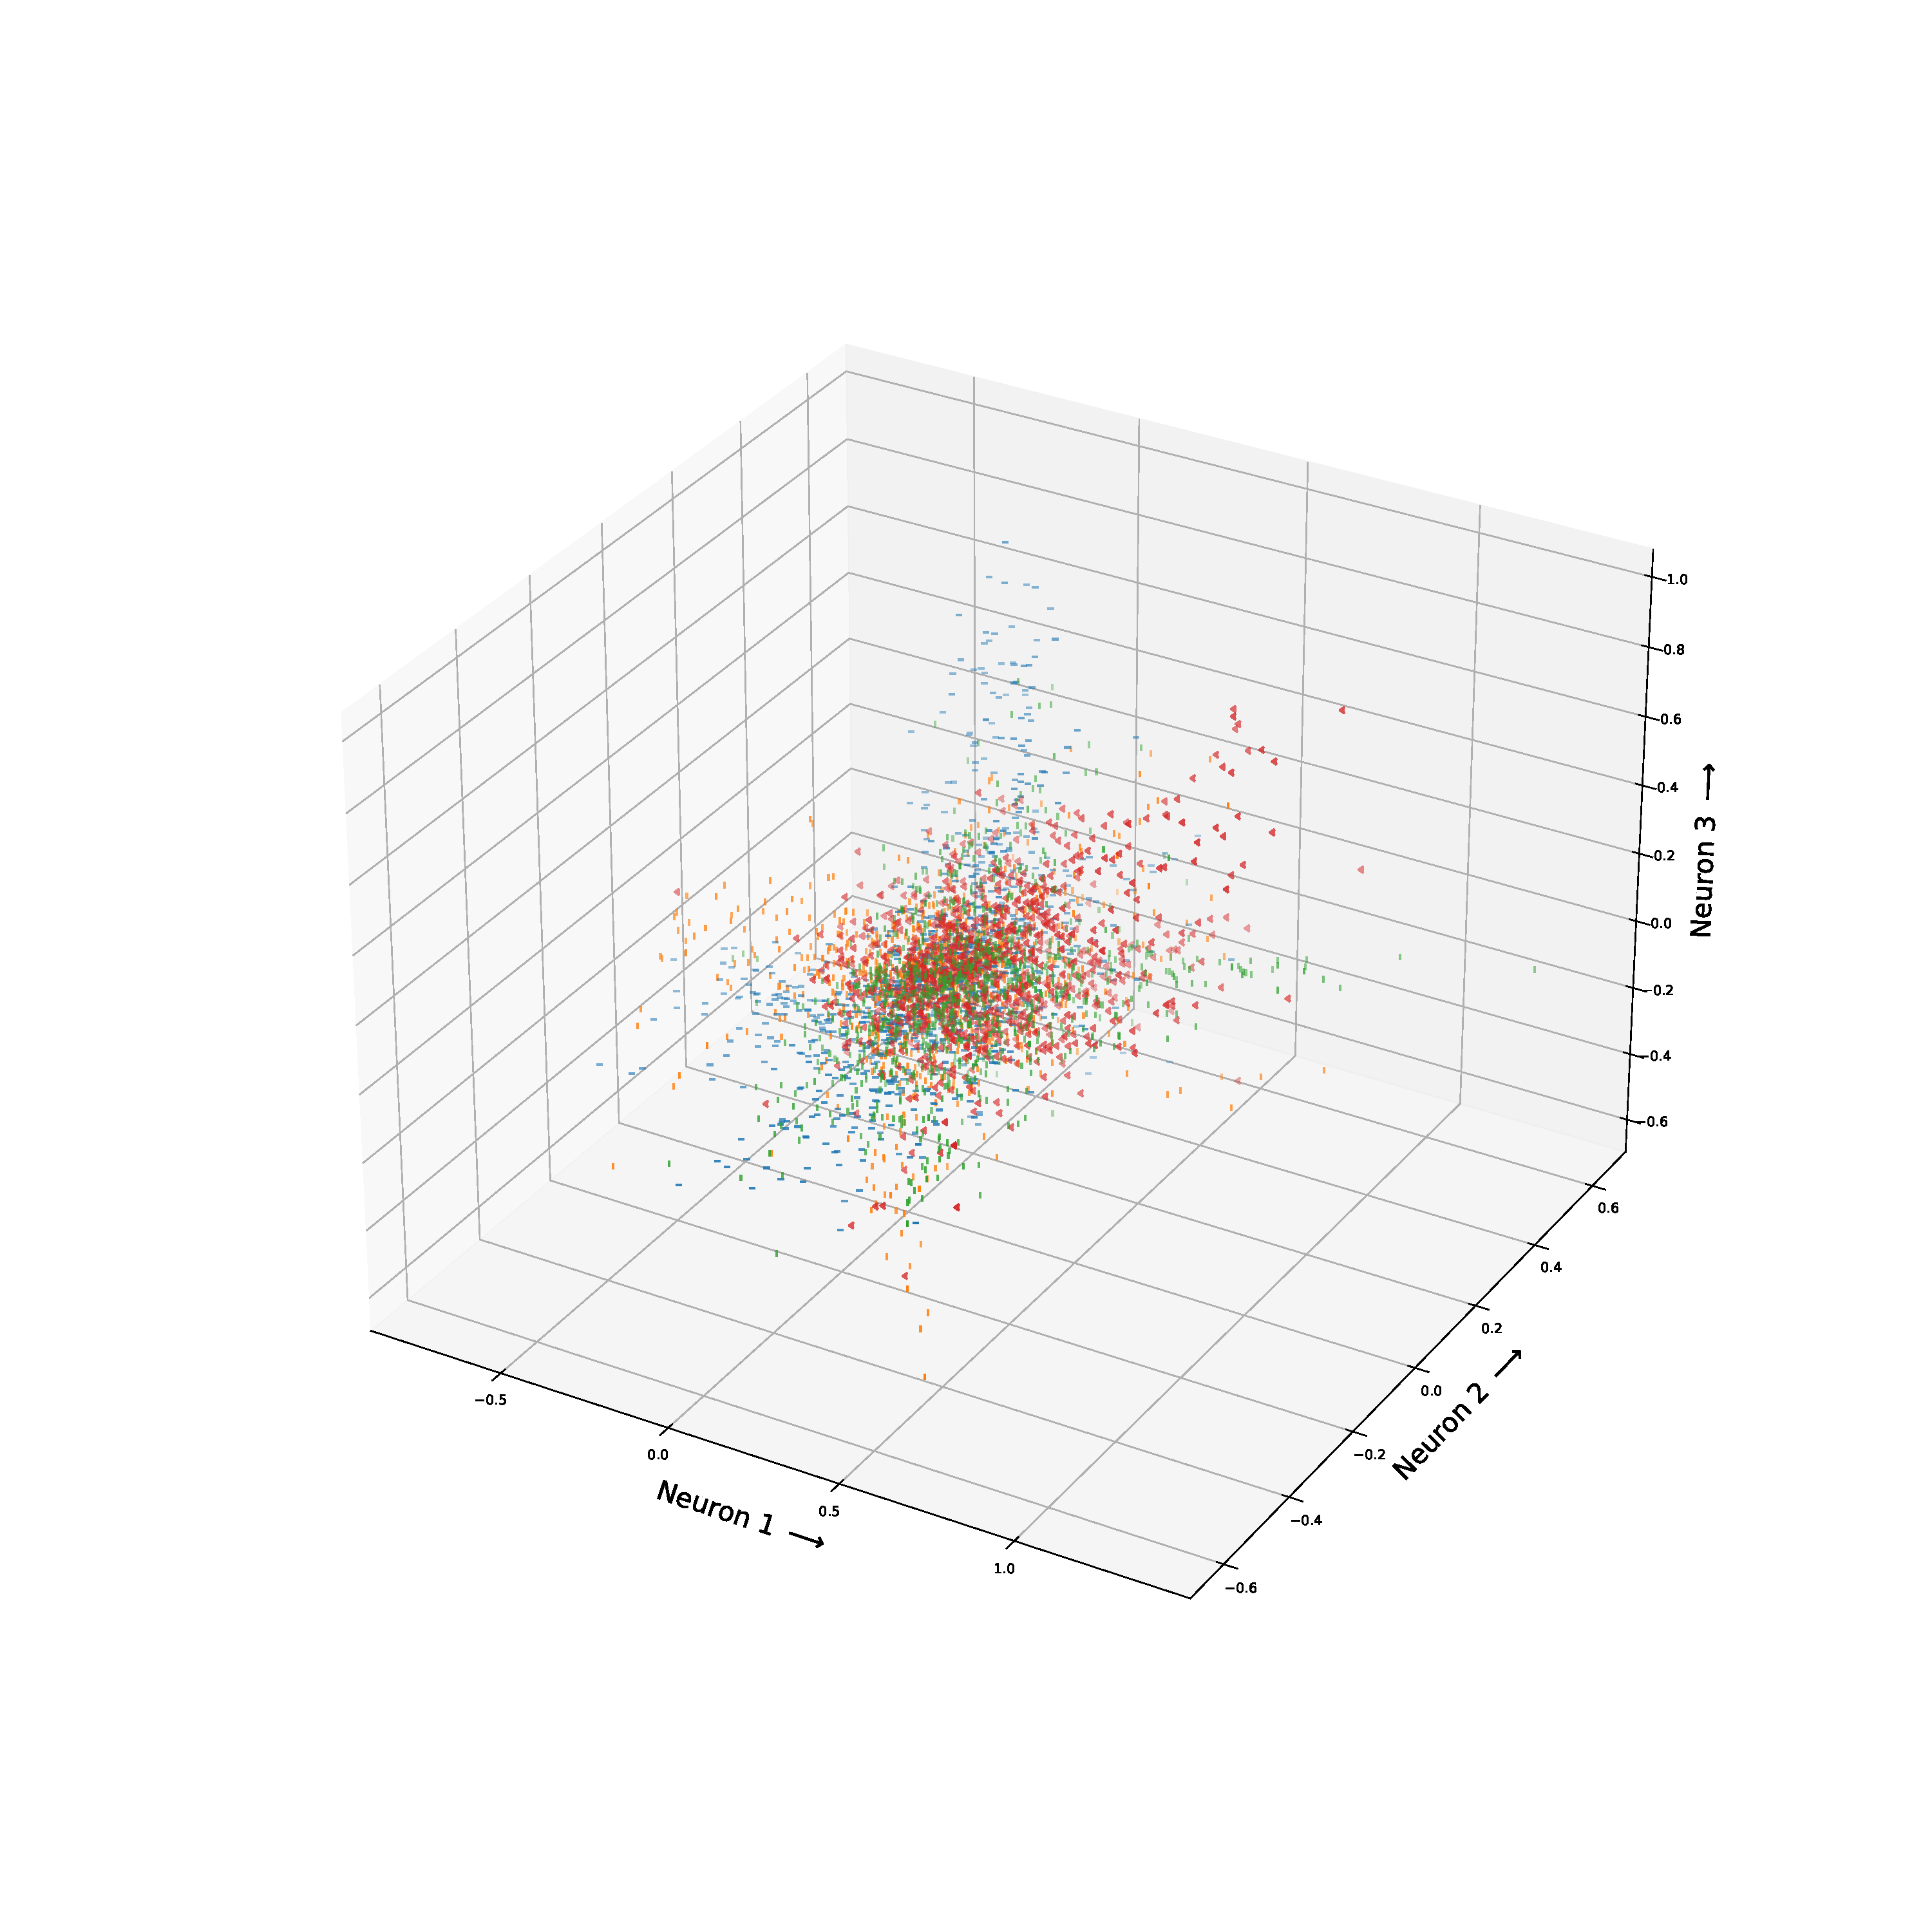
\includegraphics[width=.44\textwidth]{labeled_vs_unlabeled_point_cloud/mmd_epoch0.pdf}
  \hspace{.1cm}
  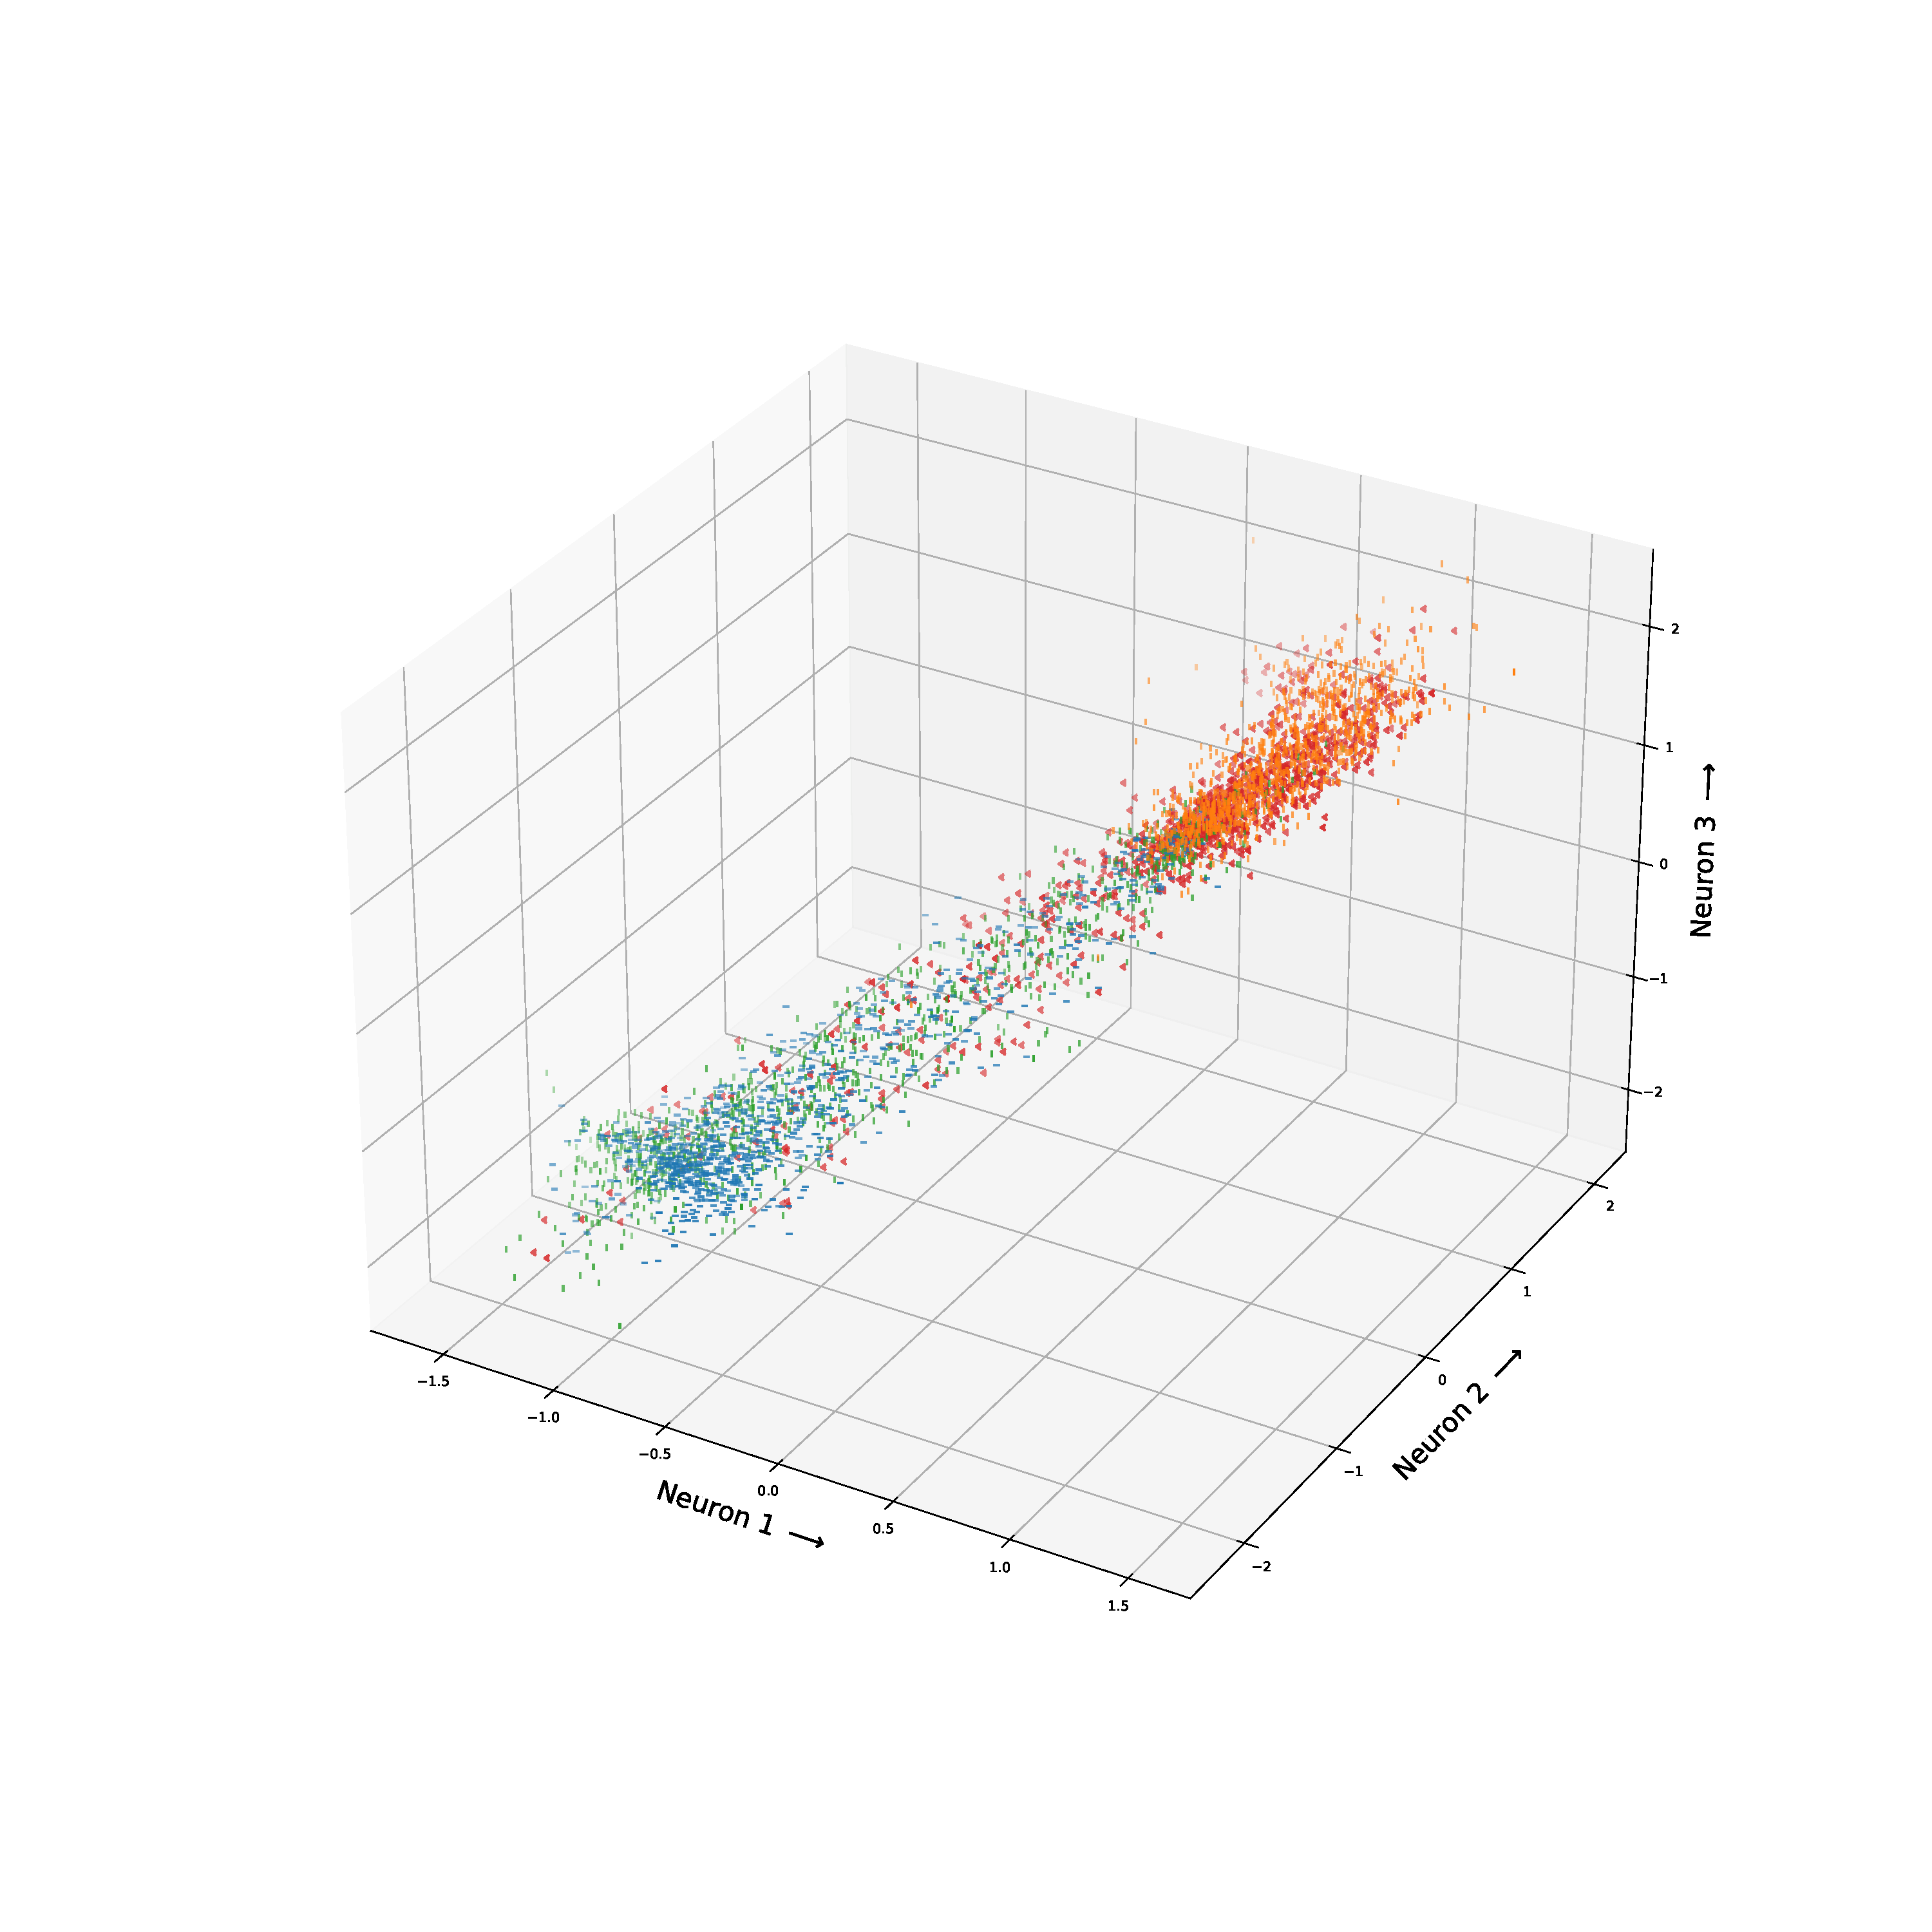
\includegraphics[width=.44\textwidth]{labeled_vs_unlabeled_point_cloud/mmd_epoch6.pdf}

  \vspace{.1cm}
  
  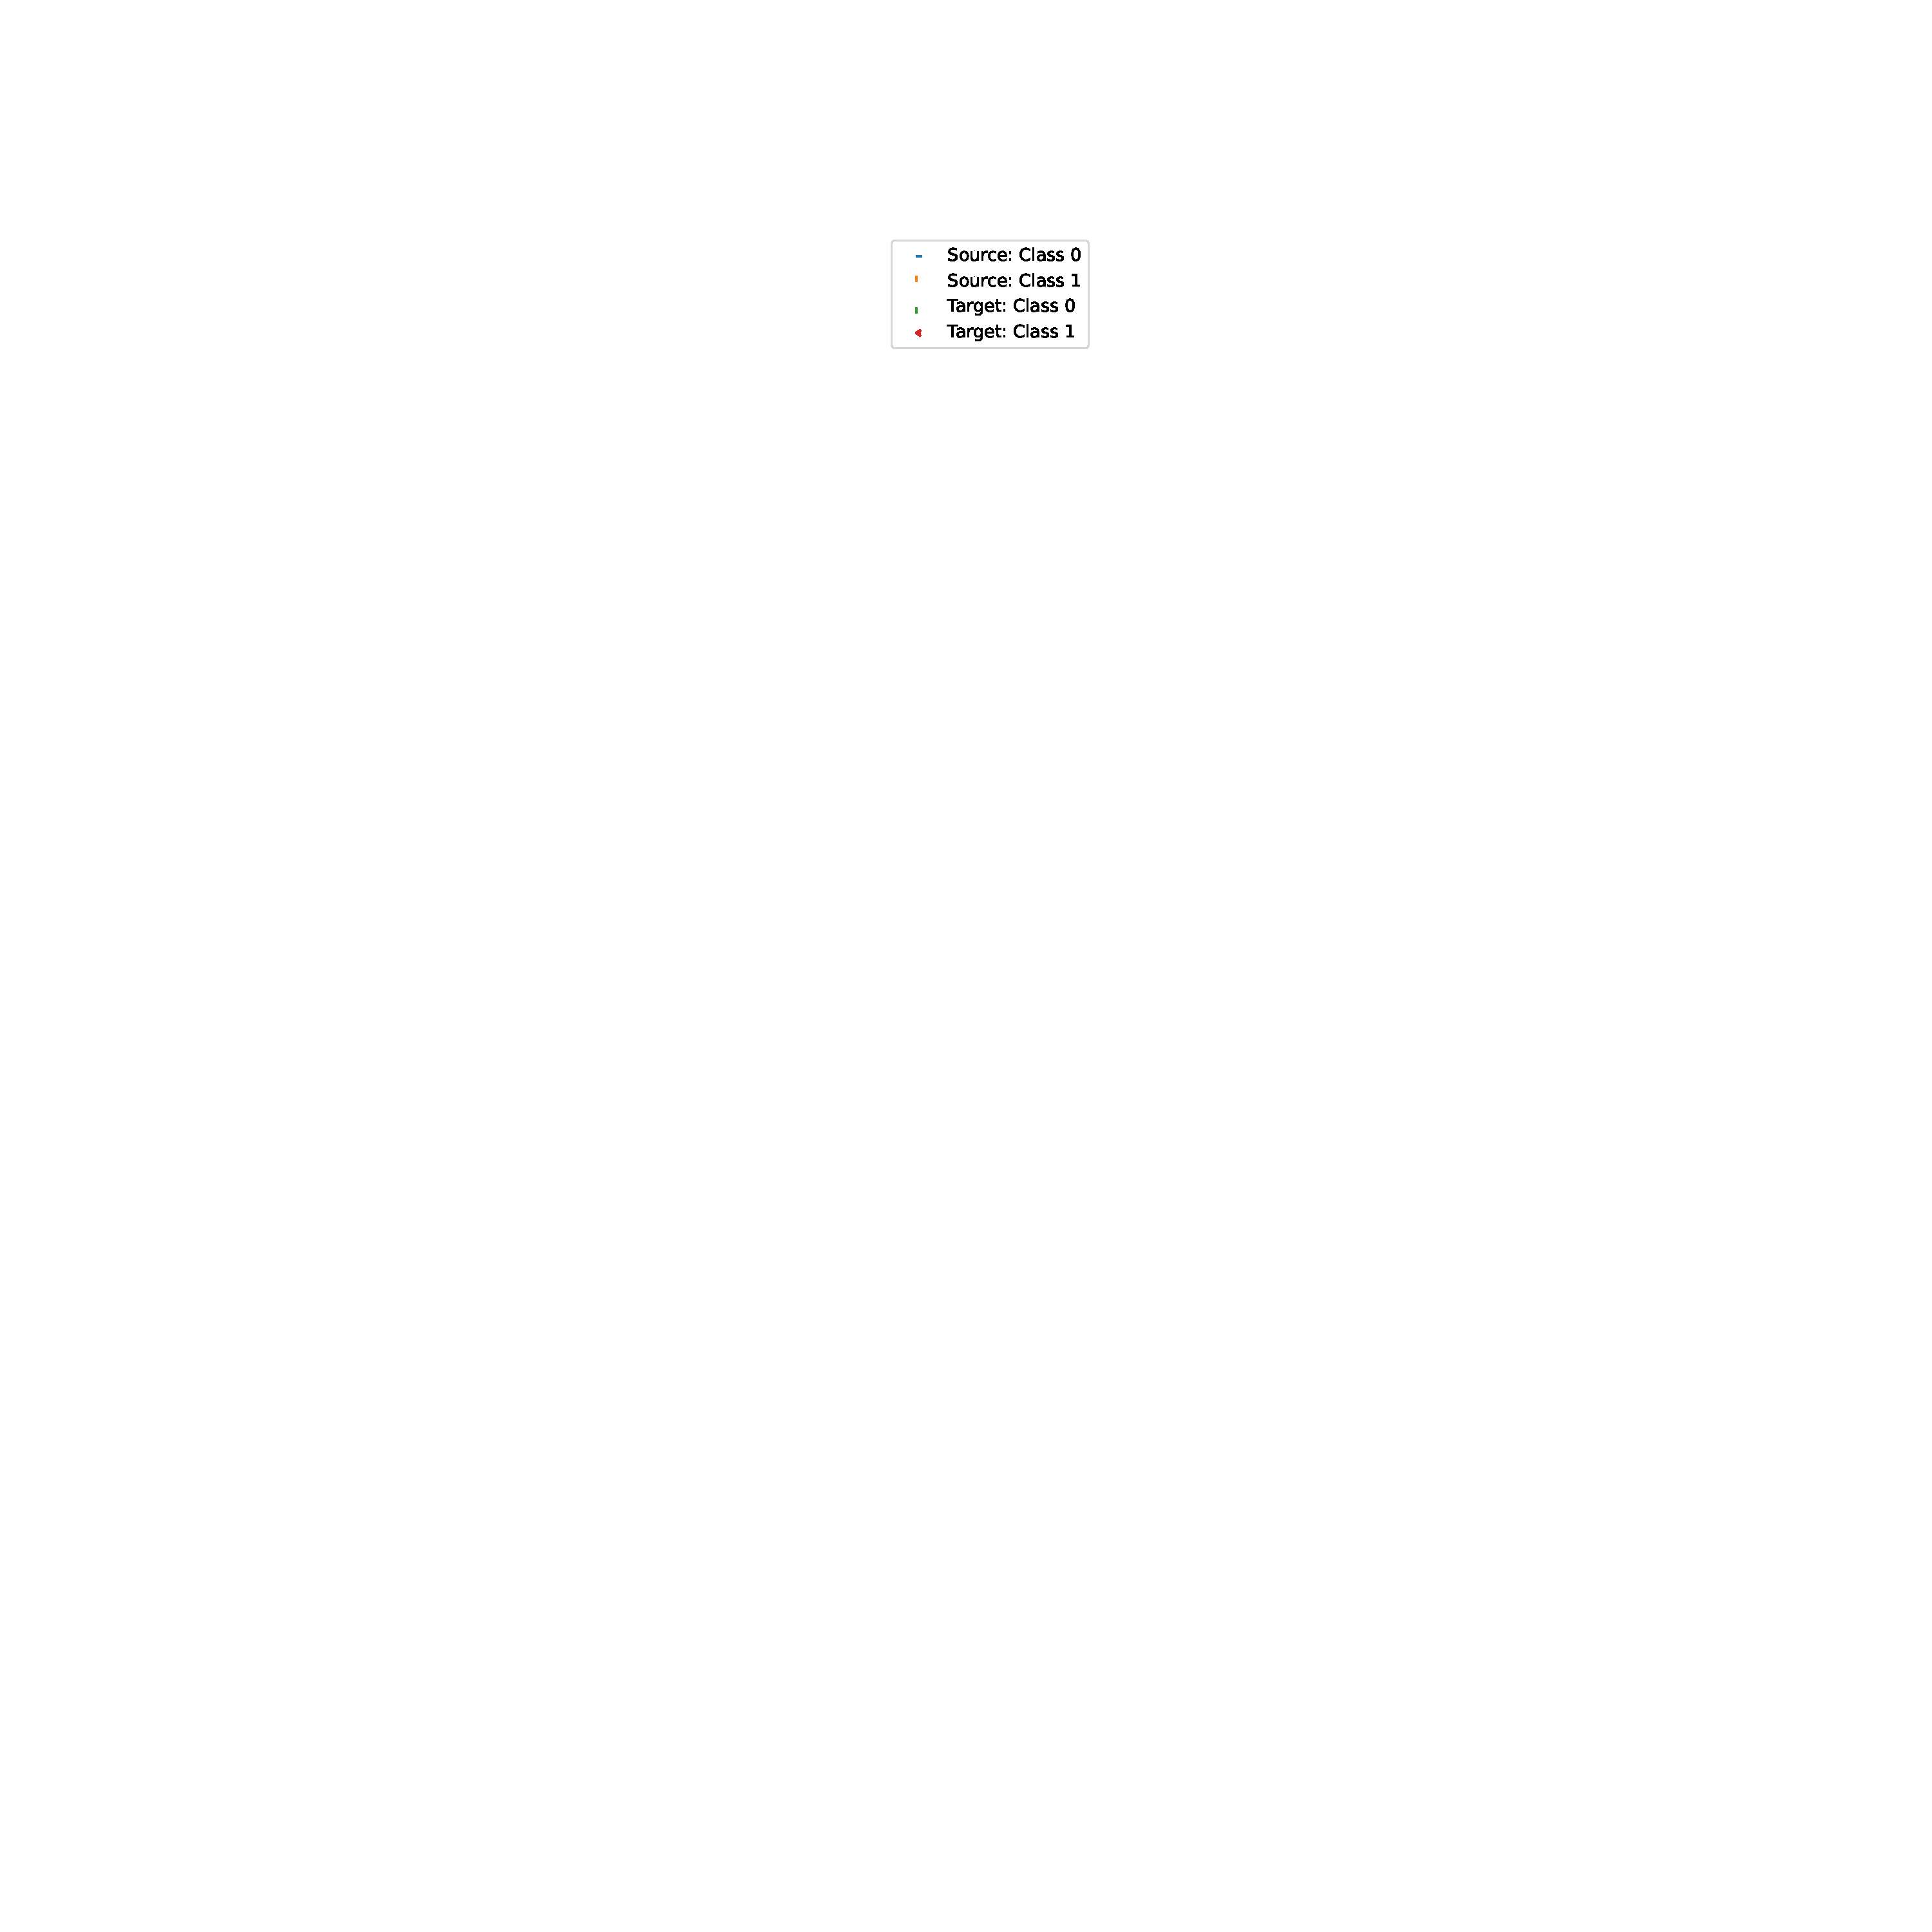
\includegraphics[width=.15\textwidth]{labeled_vs_unlabeled_point_cloud/legend.pdf}

  \caption{Data distribution: labeled (top) vs. unlabeled MMD (bottom) at epoch 0 (left) and epoch 6 (right)}
  \label{fig:point_cloud_labeled_unlabeled_mmd}
\end{figure}

\subsection{Influence of latent feature space choice in MMD loss}
\label{cnn_mmd_dummy}
This section analyzes the influence of applying the MMD loss in different latent feature maps of the CNN and classifier. The "regular FC MMD" loss calculates the source and target discrepancy from the three latent feature maps in the classifier (flattened output of CNN, FC1, FC2). The "regular FC + CNN MMD" loss additionally considers the feature maps of the three convolutional layers in the CNN (Conv 1, Conv 2 and Conv 3). The accuracy, the source cross-entropy and MMD loss during the training process are shown in fig. \ref{fig:accuracy_cnn_and_no_cnn_mmd} and fig. \ref{fig:loss_cnn_and_no_cnn_mmd}. The accuracies in source and target domain are higher when including the CNN feature maps into the MMD loss. Besides that, including the CNN feature maps in the MMD loss increases the stability of the training. The losses, as well as the accuracies, converge faster and smoother.

\begin{figure}[H]
  \centering
  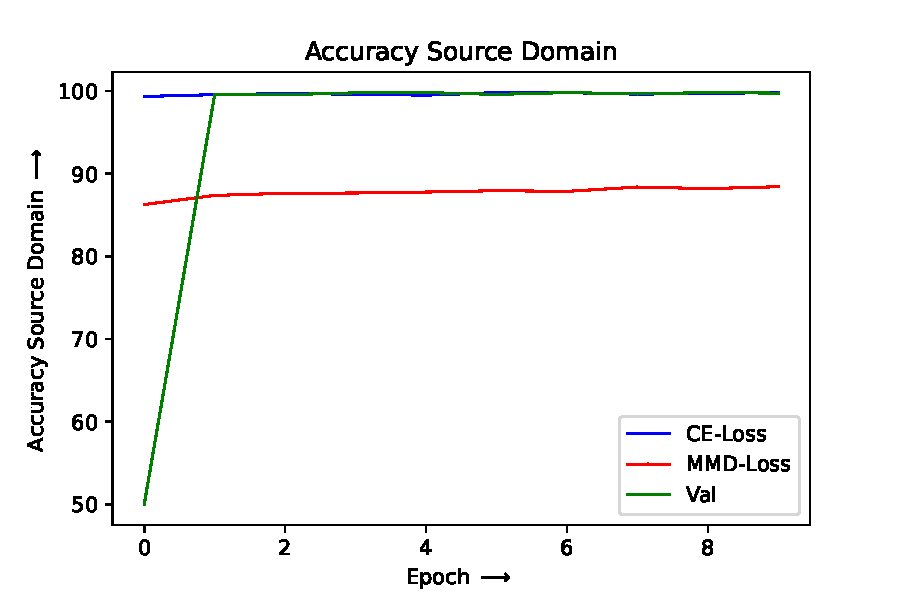
\includegraphics[width=.47\textwidth]{plots_CNN_MMD/Accuracy_Source_Domain_CNN_MMD.pdf}
  \hspace{.3cm}
  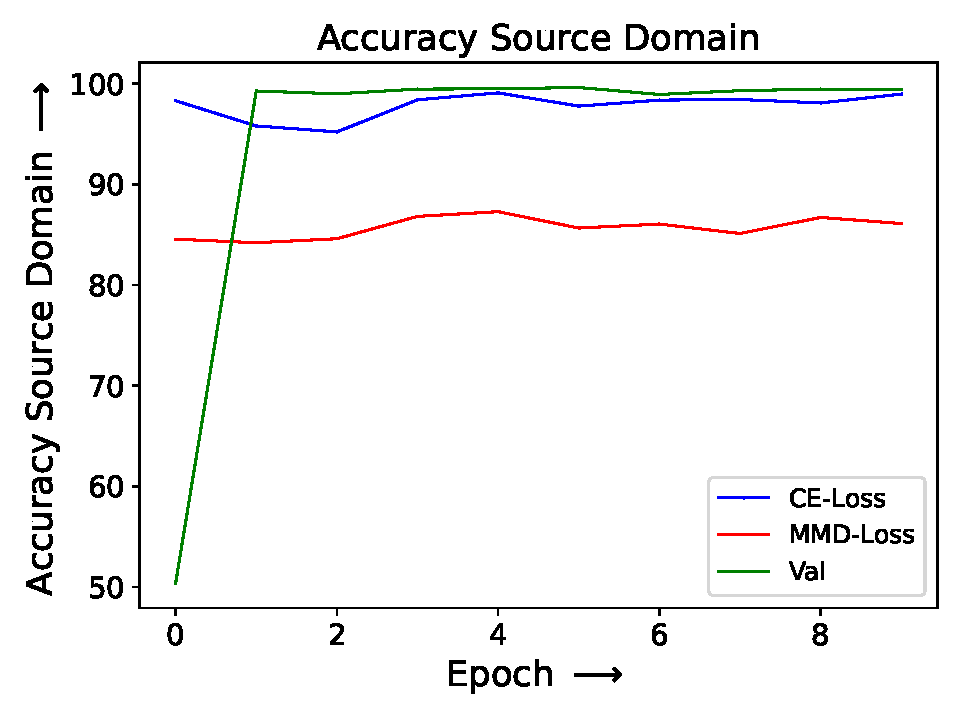
\includegraphics[width=.47\textwidth]{plots_CNN_MMD/Accuracy_Source_Domain_FC_MMD.pdf}

  \vspace{.1cm}

  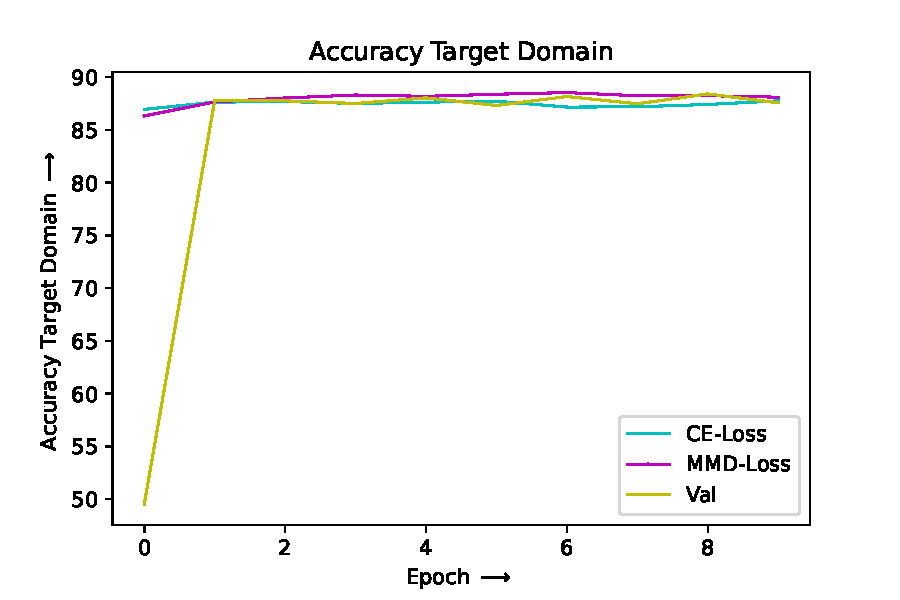
\includegraphics[width=.47\textwidth]{plots_CNN_MMD/Accuracy_Target_Domain_CNN_MMD.pdf}
  \hspace{.1cm}
  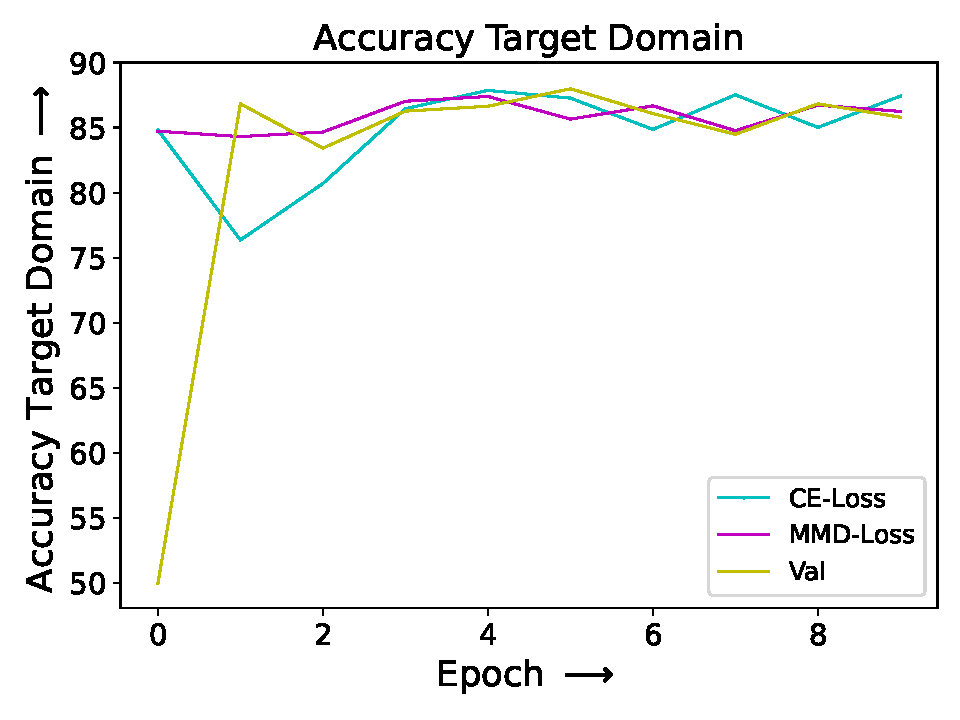
\includegraphics[width=.47\textwidth]{plots_CNN_MMD/Accuracy_Target_Domain_FC_MMD.pdf}

  \caption{Accuracy curves of regular CNN MMD Loss (left) and regular FC MMD Loss (right)}
  \label{fig:accuracy_cnn_and_no_cnn_mmd}
\end{figure}

\begin{figure}[H]
  \centering
  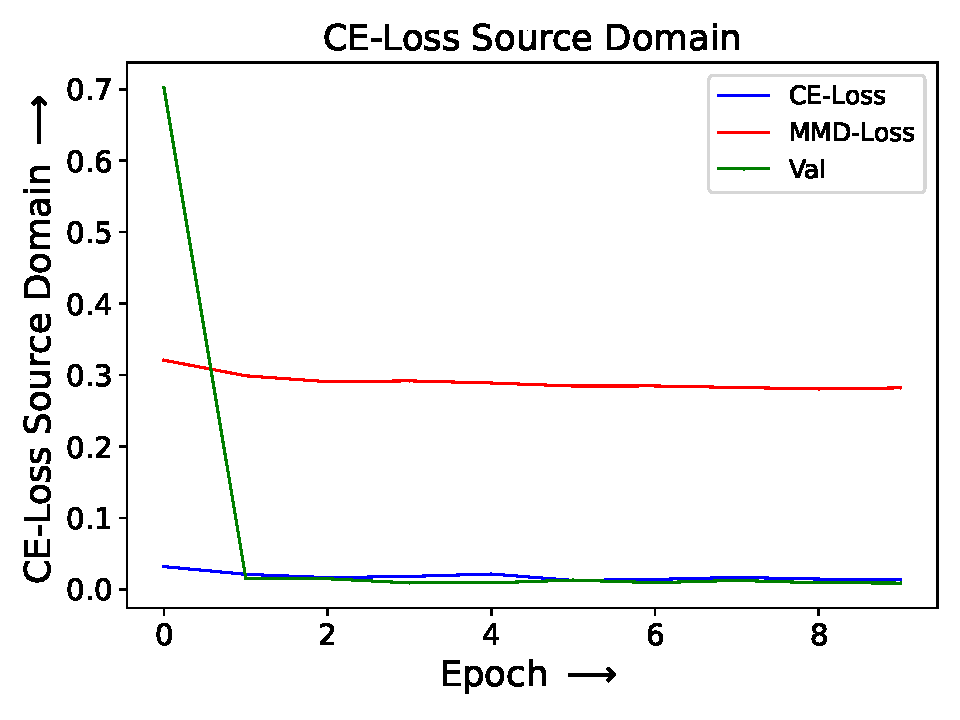
\includegraphics[width=.47\textwidth]{plots_CNN_MMD/CE_Loss_Source_Domain_CNN_MMD.pdf}
  \hspace{.3cm}
  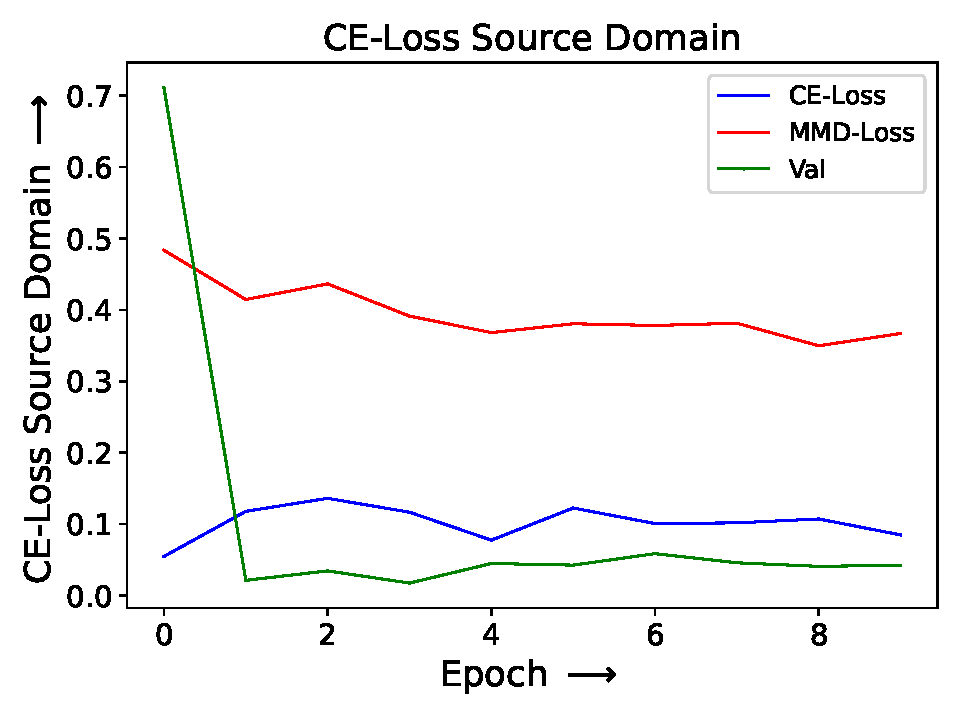
\includegraphics[width=.47\textwidth]{plots_CNN_MMD/CE_Loss_Source_Domain_FC_MMD.pdf}

  \vspace{.1cm}

  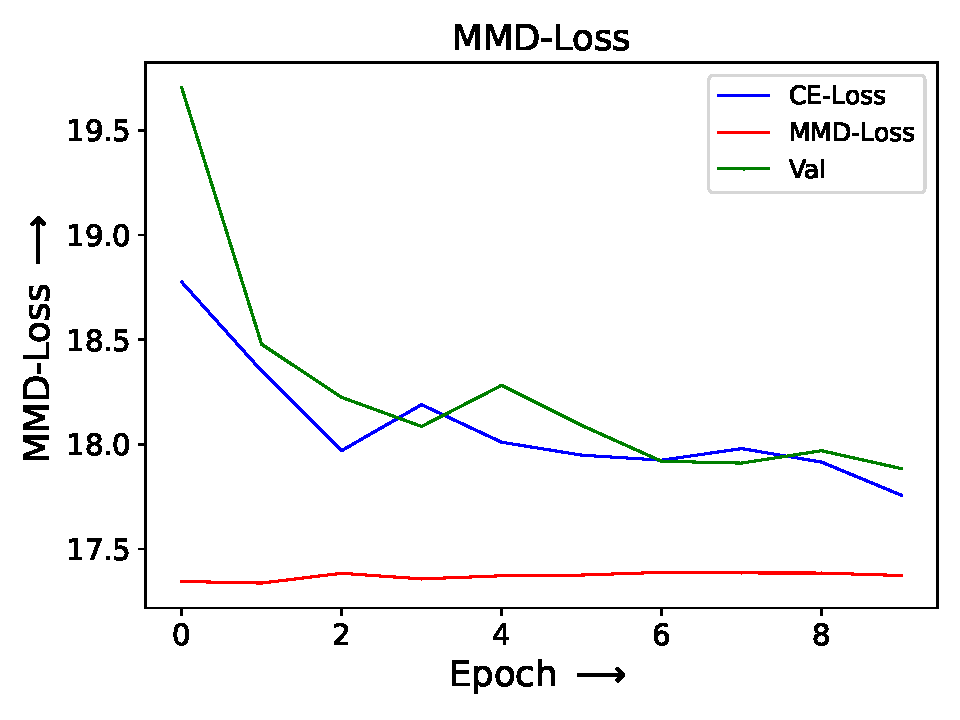
\includegraphics[width=.47\textwidth]{plots_CNN_MMD/MMD_Loss_CNN_MMD.pdf}
  \hspace{.1cm}
  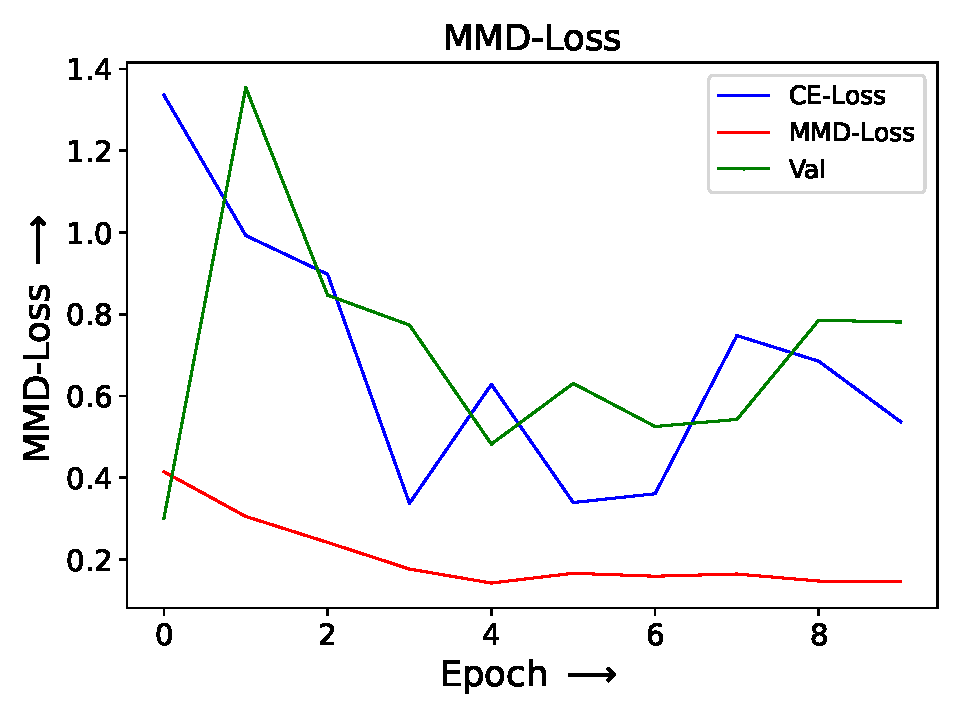
\includegraphics[width=.47\textwidth]{plots_CNN_MMD/MMD_Loss_FC_MMD.pdf}

  \caption{Loss curves of regular CNN MMD loss (left) and regular FC MMD loss(right)}
  \label{fig:loss_cnn_and_no_cnn_mmd}
\end{figure}

By passing data through the model, features with varying levels of abstraction are extracted. Supervising the domain discrepancy in feature maps of different abstraction levels seems reasonable. Generally, shallow layers in neural network extract more global and deeper more task-specific features. Deeper layers often suffer from stronger domain-dependencies. Since each layer in a neural network influences subsequent layers, it makes sense to apply the MMD loss early in the network. Reducing the domain discrepancy in shallow layers makes the network extract more domain-invariant features in all following layers as well. Especially in challenging tasks with strong domain discrepancies, it is reasonable to intervene early. Reducing the domain discrepancy just in the final layers of the model leads to a less stable and smooth optimizations. Potentially, the MMD and source cross-entropy loss tend to be more contradicting when applied in these layers. The two training goals, which seem to work against each other, make the optimization more fluctuating. During the optimization, different strong local minima coming from one of the two losses might be found. The model performance sometimes breaks down after some stable epochs of constant training. One has to remember calculating the regular FC + CNN MMD loss is quite expansive since the feature maps extracted from the convolutional layers are complex and high-dimensional.



\section{Real-world dataset}
In the following section the performance of different MMD-based domain adaption approaches are evaluated on the real-world ball screw dataset. The model used for this evaluation is presented in fig. \ref{fig:model_real_data}. From the 49 features in the dataset just three (\verb|'C:x_bottom'|, \verb|'C:y_bottom'|, \verb|'C:z_bottom'|) are used. For this reasons three sequences of length 1024 are fed into the CNN.

\begin{figure}[H]
  \centering
  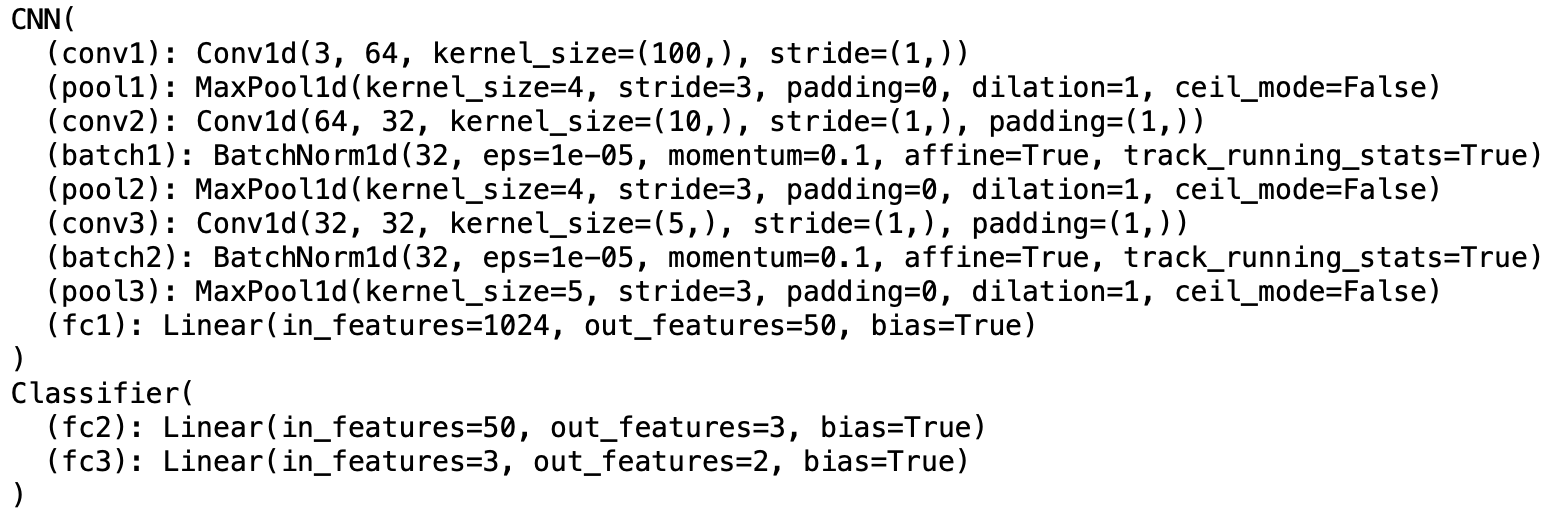
\includegraphics[width=1.1\textwidth]{model_real_data}
  \caption {MMD Model for real data} \label{fig:model_real_data}
\end{figure}


On the real machine dataset the three approaches regular FC + CNN MMD loss,  regular FC MMD and no MMD loss are evaluated. The accuracies on the source and target domain are visualized in fig. \ref{fig:accuracy_real_world}. In each figure three curves are presented representing different phases of the training. During the MMD Loss phase the whole model consisting of CNN and classifier are optimized with a weighted average of MMD and cross entropy loss. In the CE-Loss phase just the classifier is optimized according to a cross-entropy loss. During both phases an ADAM optimizer with a learning rate of 1e-2, beta1 of 0.9 and beta2 of 0.99 is used . In the val phase the model is evaluated. Before the training the data is split for these three phases accordingly (MMD-Loss: 60\%, CE-Loss: 20\%, Val: 20\%). Therefore all experiments follow a proper train validation split. It becomes obvious that the accuracies achieved on the validation set of the target domain were able to be increased with about 10\% by using the two MMD variations. The MMD and cross entropy loss seems to be decreased more smoothly when including CNN features into the MMD loss for the optimization of the model. Also the accuracy achieved on the target validation set achieved the regular FC + CNN MMD loss beat the one achieved with the regular FC MMD loss. Without using any MMD loss the model performance on the target domain could be increased by just around 2\%. When using the regular FC MMD loss sometimes the performance of the model breaks down  little bit. Often times this can be seen in the accuracy of the target and source domain. An example for this phenomena can be seen in fig. \ref{fig:accuracy_real_world} when looking at the accuracies of regular FC MMD (middle). In epoch ~27 the accuracy breaks down on the target and source domain. Especially during the combined training with the MMD and cross entropy loss this effect becomes especially obvious. Like mentioned in previous chapters this shows that when not including the latent features of the CNN in the MMD loss the cross entropy and MMD loss seem to work against each other, which makes the optimization less stable.

\begin{figure}[H]
  \centering
  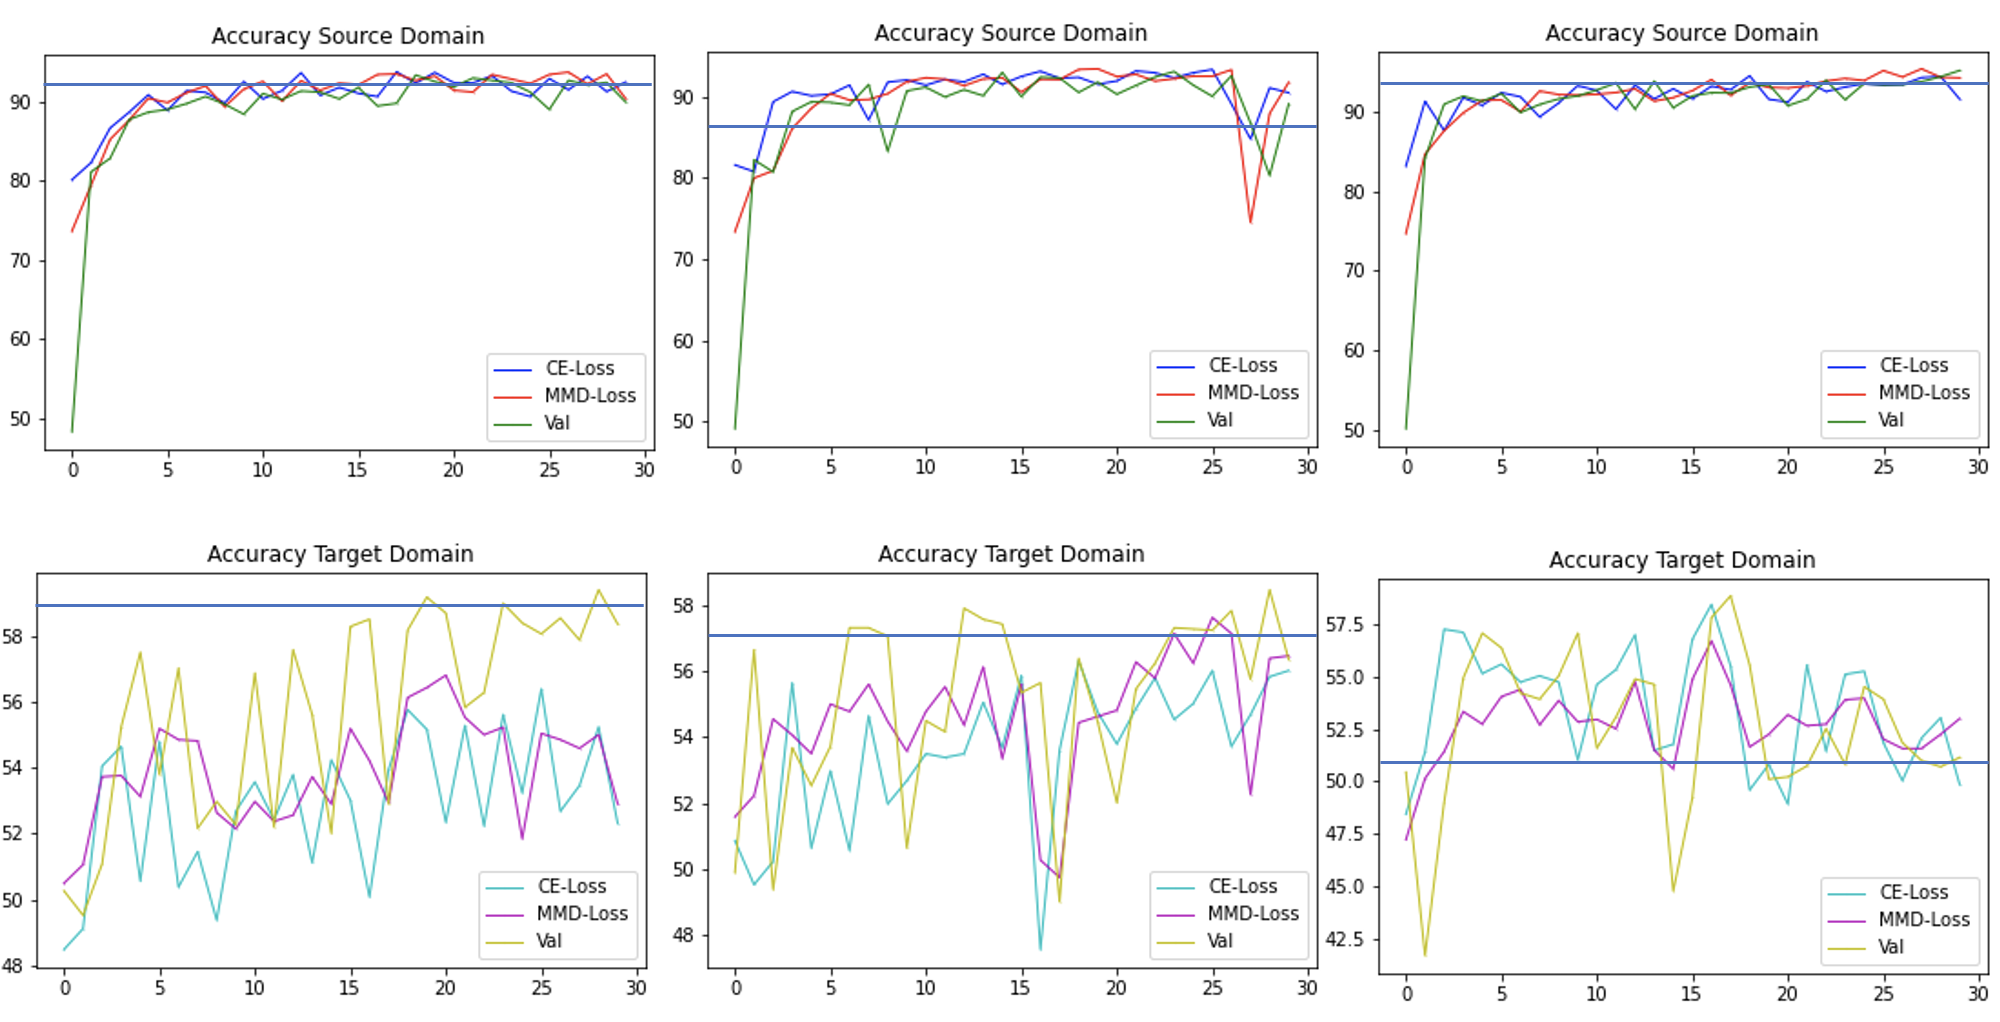
\includegraphics[width=1.1\textwidth]{accuracy_real_world}
  \caption {Accuracies for model training with Regular FC + CNN MMD loss (left), Regular FC MMD (middle) and No MMD loss (right)} \label{fig:accuracy_real_world}
\end{figure}


\begin{figure}[H]
  \centering
  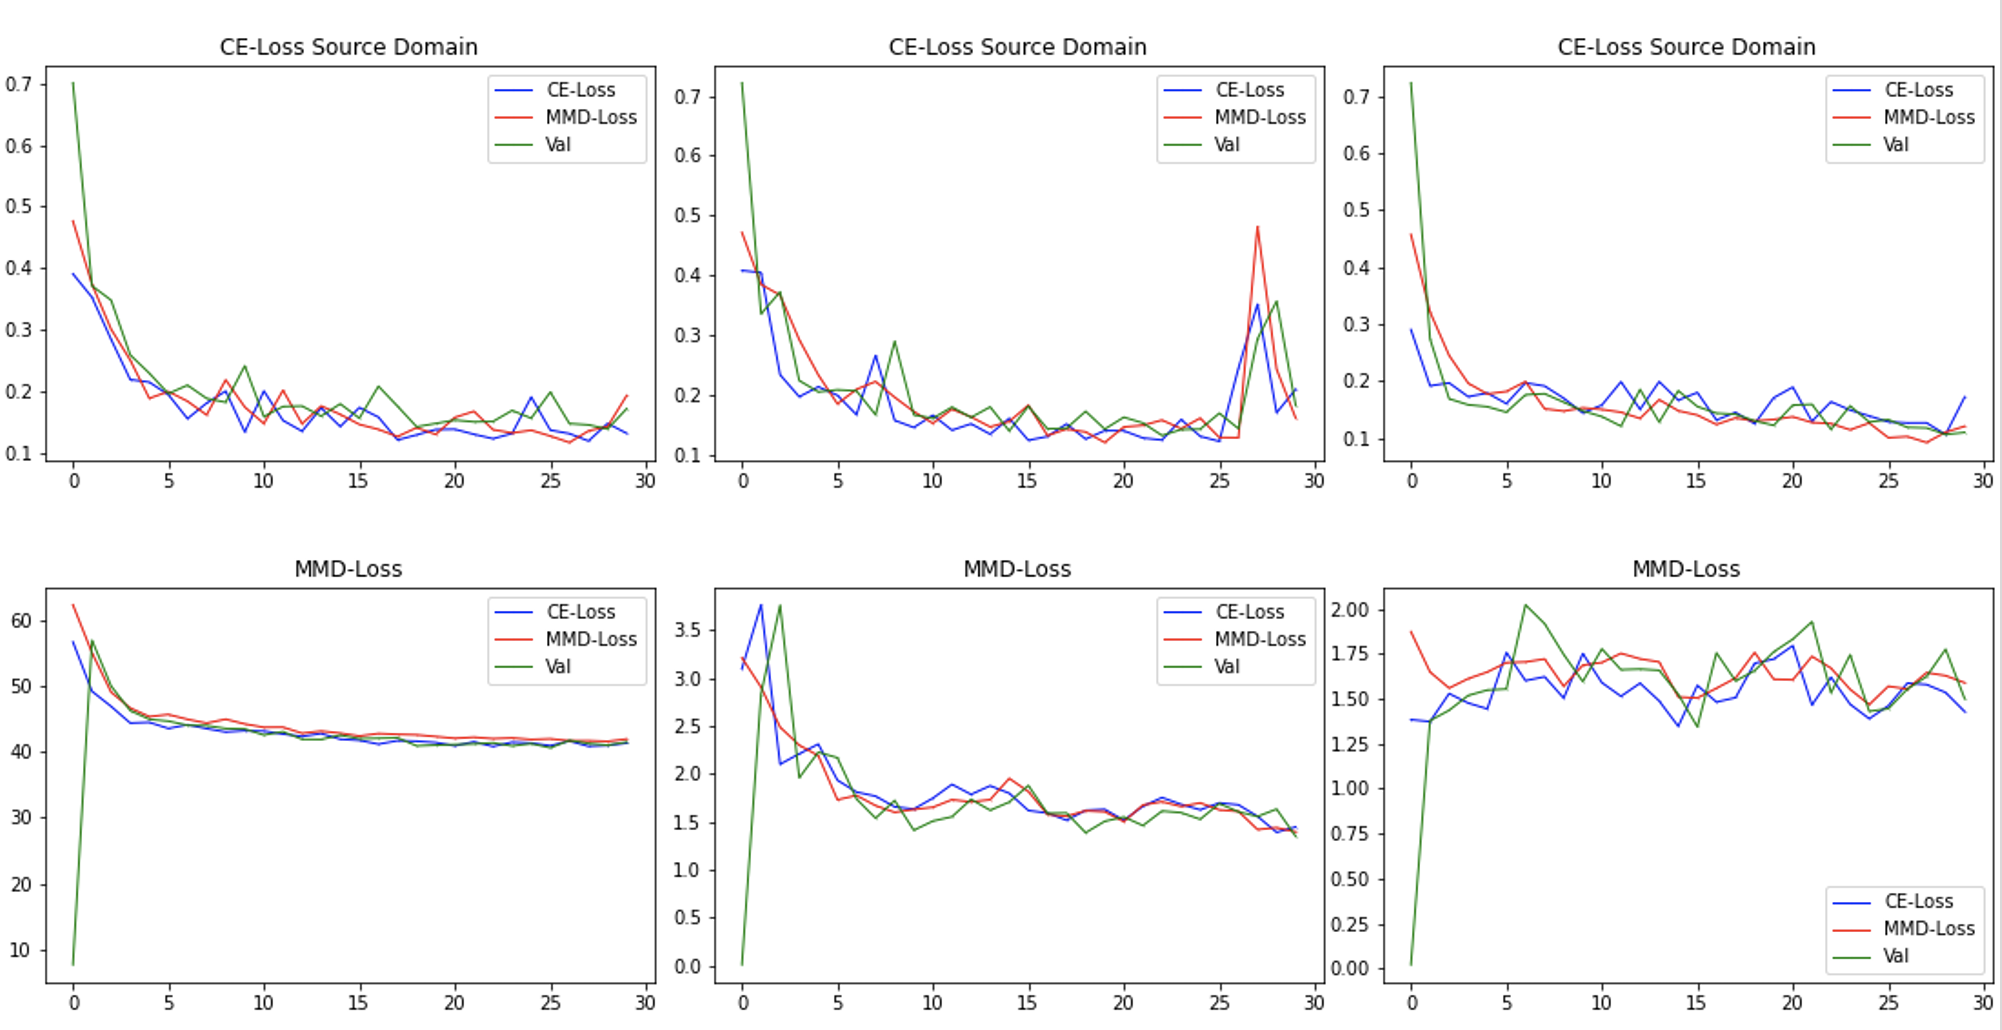
\includegraphics[width=1.1\textwidth]{loss_real_world}
  \caption {Loss for model training with Regular FC + CNN MMD loss (left), Regular FC MMD (middle) and No MMD loss} \label{fig:loss_real_world}
\end{figure}


In fig. the development of the source domain cross entropy MMD loss is shown. It can be seen, that the hyperparameter GAMMA was picked well, such that the MMD as well as the source cross entropy loss were able to be reduced smoothly throughout the trainings process. 


Unfortunately the MMD loss could just minimize the domain discrepancy by a little. The domain discrepancy problem couldn't be solved completely. Still the idea of the MMD loss becomes more clear in the experiments. Also the positive effect of the MMD loss for the training is obvious. For the complex multi-dimensional dataset the MMD loss is probably not sophisticated enough to detect and effectively fight the domain discrepancy.
